\chapter{基于图神经网络的多目标跟踪算法研究}
在前两章中,本文系统回顾了多目标跟踪任务的研究背景,并重点分析了图神经网络(GNN)在轨迹关联建模中的优势。现有基于图的跟踪方法多采用“边分类”范式,通过构建帧间稠密图判断连边关系,但存在图结构冗余、计算复杂度高的问题,往往难以满足在线应用对实时性的严苛要求。

针对上述局限性,本章提出一种双图协同关联的在线跟踪器(Dual-Graph Collaborative Tracker,DGCTracker)。该方法摒弃了传统的帧间稠密构图方式,转而采用KNN自适应稀疏构图策略,将图规模显著降低。核心思想是通过构建静态图(Static Graph) 与动态图(Dynamic Graph) ,
分别从空间几何分布与语义拓扑结构两个互补视角提取判别性节点嵌入,从而在复杂场景下实现稳健的在线轨迹关联。

本章结构安排如下:首先,在\ref{sec:ch3_1}节中对在线多目标跟踪任务进行形式化建模,明确本文的优化目标;随后,\ref{sec:ch3_2}节详细介绍DGCTracker的整体框架,包括稀疏图构建、双图特征提取与融合、跨帧关联匹配及数据增强策略;
接着,\ref{sec:ch3_3}节阐述轨迹状态管理策略;\ref{sec:ch3_4}节通过在MOT16/17基准上的实验全面验证所提方法的有效性;最后,\ref{sec:ch3_5}节对本章工作进行总结。
\section{在线多目标跟踪的问题建模}
\label{sec:ch3_1}
\subsection{在线跟踪任务描述}
在“先检测后跟踪”(Tracking-by-Detection)的主流范式下,在线多目标跟踪任务可被形式化为一个逐帧的数据关联问题。其核心目标是在不依赖未来帧信息的前提下,将当前帧的检测结果与历史轨迹进行准确匹配,从而为每个目标建立连续、稳定的身份标识(Identity,ID)。

具体而言,设第$t-1$时刻已维护的轨迹集合为$\mathcal{L}^{t-1}=\{l_i^{t-1}\}_{i=1}^{N_{t-1}}$,其中$N_{t-1}$表示当前活跃轨迹的数量;在当前时刻$t$,前端检测器输出一组检测结果$\mathcal{D}^t = \{d_j^t\}_{j=1}^{M_t}$,其中$M_t$为当前帧的检测目标数量。
每一条轨迹$l_i^{t-1}$和检测目标$d_j^t$均包含其对应的空间位置信息$(x,y,w,h)$,检测置信度和原始像素特征。

根据互斥匹配原则,每个检测至多与一条轨迹关联,反之亦然。同时允许部分目标未被匹配以兼容轨迹的新生或消失。因此,在线跟踪任务可建模为带互斥约束的最优化问题:通过计算轨迹-检测亲和度矩阵$S \in \mathbb{R}^{N_{t-1}\times M_t}$,求解双射约束下的最优关联矩阵$A_t = (a_{ij}^t)$,使得总匹配置信度最大化:
\begin{equation}
\begin{aligned}
\max_{A_t} \quad 
& \left[ \langle A_t, S \rangle_F = \sum_{i=1}^{N_{t-1}} \sum_{j=1}^{M_t} a_{ij}^t \, \phi\!\left(l_i^{t-1}, d_j^{t}\right) \right] \\
\text{s.t.} \quad
& \left\{
\begin{aligned}
& \sum_{i=1}^{N_{t-1}} a_{ij}^t \le 1,
&& \forall j = 1,\ldots,M_t, \\
& \sum_{j=1}^{M_t} a_{ij}^t \le 1,
&& \forall i = 1,\ldots,N_{t-1}, \\
& a_{ij}^t \in \{0,1\},
&& \forall i,j .
\end{aligned}
\right.
\end{aligned}
\label{equ:online_matching}
\end{equation}

其中,$\langle \cdot, \cdot \rangle_F$代表Frobenius内积,$\phi(\cdot,\cdot)$表示轨迹与检测间的亲和度度量函数,二元决策变量$a_{ij}^t$表征匹配状态:当且仅当轨迹$l_i^{t-1}$与检测$d_j^t$的被判定为同一目标(即匹配成功)时,$a_{ij}^t=1$,否则$a_{ij}^t=0$。
\subsection{数据关联问题的图建模}
为求解式\ref{equ:online_matching}所描述的轨迹–检测匹配问题,关键在于如何有效建模轨迹与检测目标之间的亲和度函数 $\phi(\cdot,\cdot)$,从而获得可靠的轨迹–检测亲和度评估。

在传统非图方法中,亲和度函数通常基于手工设计的几何度量或外观特征的线性组合来构建。例如,经典的SORT算法\cite{sort} 
主要依赖卡尔曼滤波(Kalman Filter)预测位置与当前检测框之间的交并比(IoU)来衡量几何一致性;而DeepSORT算法进一步引入了深度外观特征,通过计算特征向量间的余弦距离并结合运动状态的马氏距离(Mahalanobis Distance)作为关联依据。
这类方法虽然高效,但将每个目标视为独立的个体进行计算,未能显式建模目标之间的空间布局关系与群体运动模式,在目标密集、相互遮挡或外观相似时容易导致匹配歧义。

为了突破上述局限,从图论的视角来看,引入图神经网络(GNN)对目标间的关系进行显式建模已成为主流趋势。
现有的在线图跟踪方法大多采用跨帧构图策略\cite{li2020graph,weng2020gnn3dmot,gcnnmatch,wang2021joint,hyun2023detection},即在相邻两帧之间建立图结构,将上一时刻的轨迹节点与当前时刻的检测节点同时纳入同一张图中,并通过边来表示潜在的匹配关系。
因此,数据关联问题可自然表述为二分图匹配(Bipartite Graph Matching)问题,其核心任务就是判断一条跨帧连边所连接的节点是否同属于一个目标。

然而,为了保证召回率,这类方法通常需要对每个轨迹节点连接多个候选检测节点,引入了大量冗余候选连边。尤其在高密度场景下,图的边数随目标数量呈平方级增长,
不仅显著增加计算复杂度,还因噪声边的干扰而降低匹配精度。此外,此类构图方式将关联决策完全依赖于跨帧边的学习,忽略了帧内目标间固有的空间布局与群体结构信息,而这些上下文线索对于区分外观相似或相互遮挡的目标至关重要。
\begin{figure}[htbp]
    \centering
    \includegraphics[width=15cm]{chapter3/1.png}
    \caption{\label{fig:ch3_1}两种图构建方式对比示例}
\end{figure}

基于上述分析,本文将数据关联问题建模为一般图匹配(General Graph Matching)问题。如\autoref{fig:ch3_1}所示,本文摒弃了跨帧连接的二分图方式(如\autoref{fig:ch3_1}(a)),转而
采用帧内独立构图策略(如\autoref{fig:ch3_1}(b)):分别基于历史轨迹集合$\mathcal{L}^{t-1}$和当前检测集合$\mathcal{D}^{t}$构建两张独立的图$G^l$与$G^d$。
在此框架下,数据关联不再直接预测跨图连边,而是通过图神经网络分别学习两张图中节点的上下文嵌入表示,再基于节点嵌入的相似性构建亲和矩阵。
这一转变使得模型能够充分挖掘帧内目标间的几何与语义依赖关系,并将这些上下文信息编码进节点特征中,从而为跨帧匹配提供更具判别力的依据。
同时,由于图结构仅在各自集合内部构建,图规模得以显著压缩,有效缓解了高密度场景下的计算瓶颈。

\section{双图协同关联跟踪框架}
\label{sec:ch3_2}
在上一小节中,本文将在线多目标跟踪的数据关联问题形式化为一般图匹配问题,并指出通过帧内构图与节点嵌入学习,可以在降低计算复杂度的同时引入更丰富的上下文信息。本节在此基础上,详细介绍所提出的双图协同关联跟踪框架(DGCTracker)的整体设计与实现流程。
\begin{figure}[htbp]
    \centering
    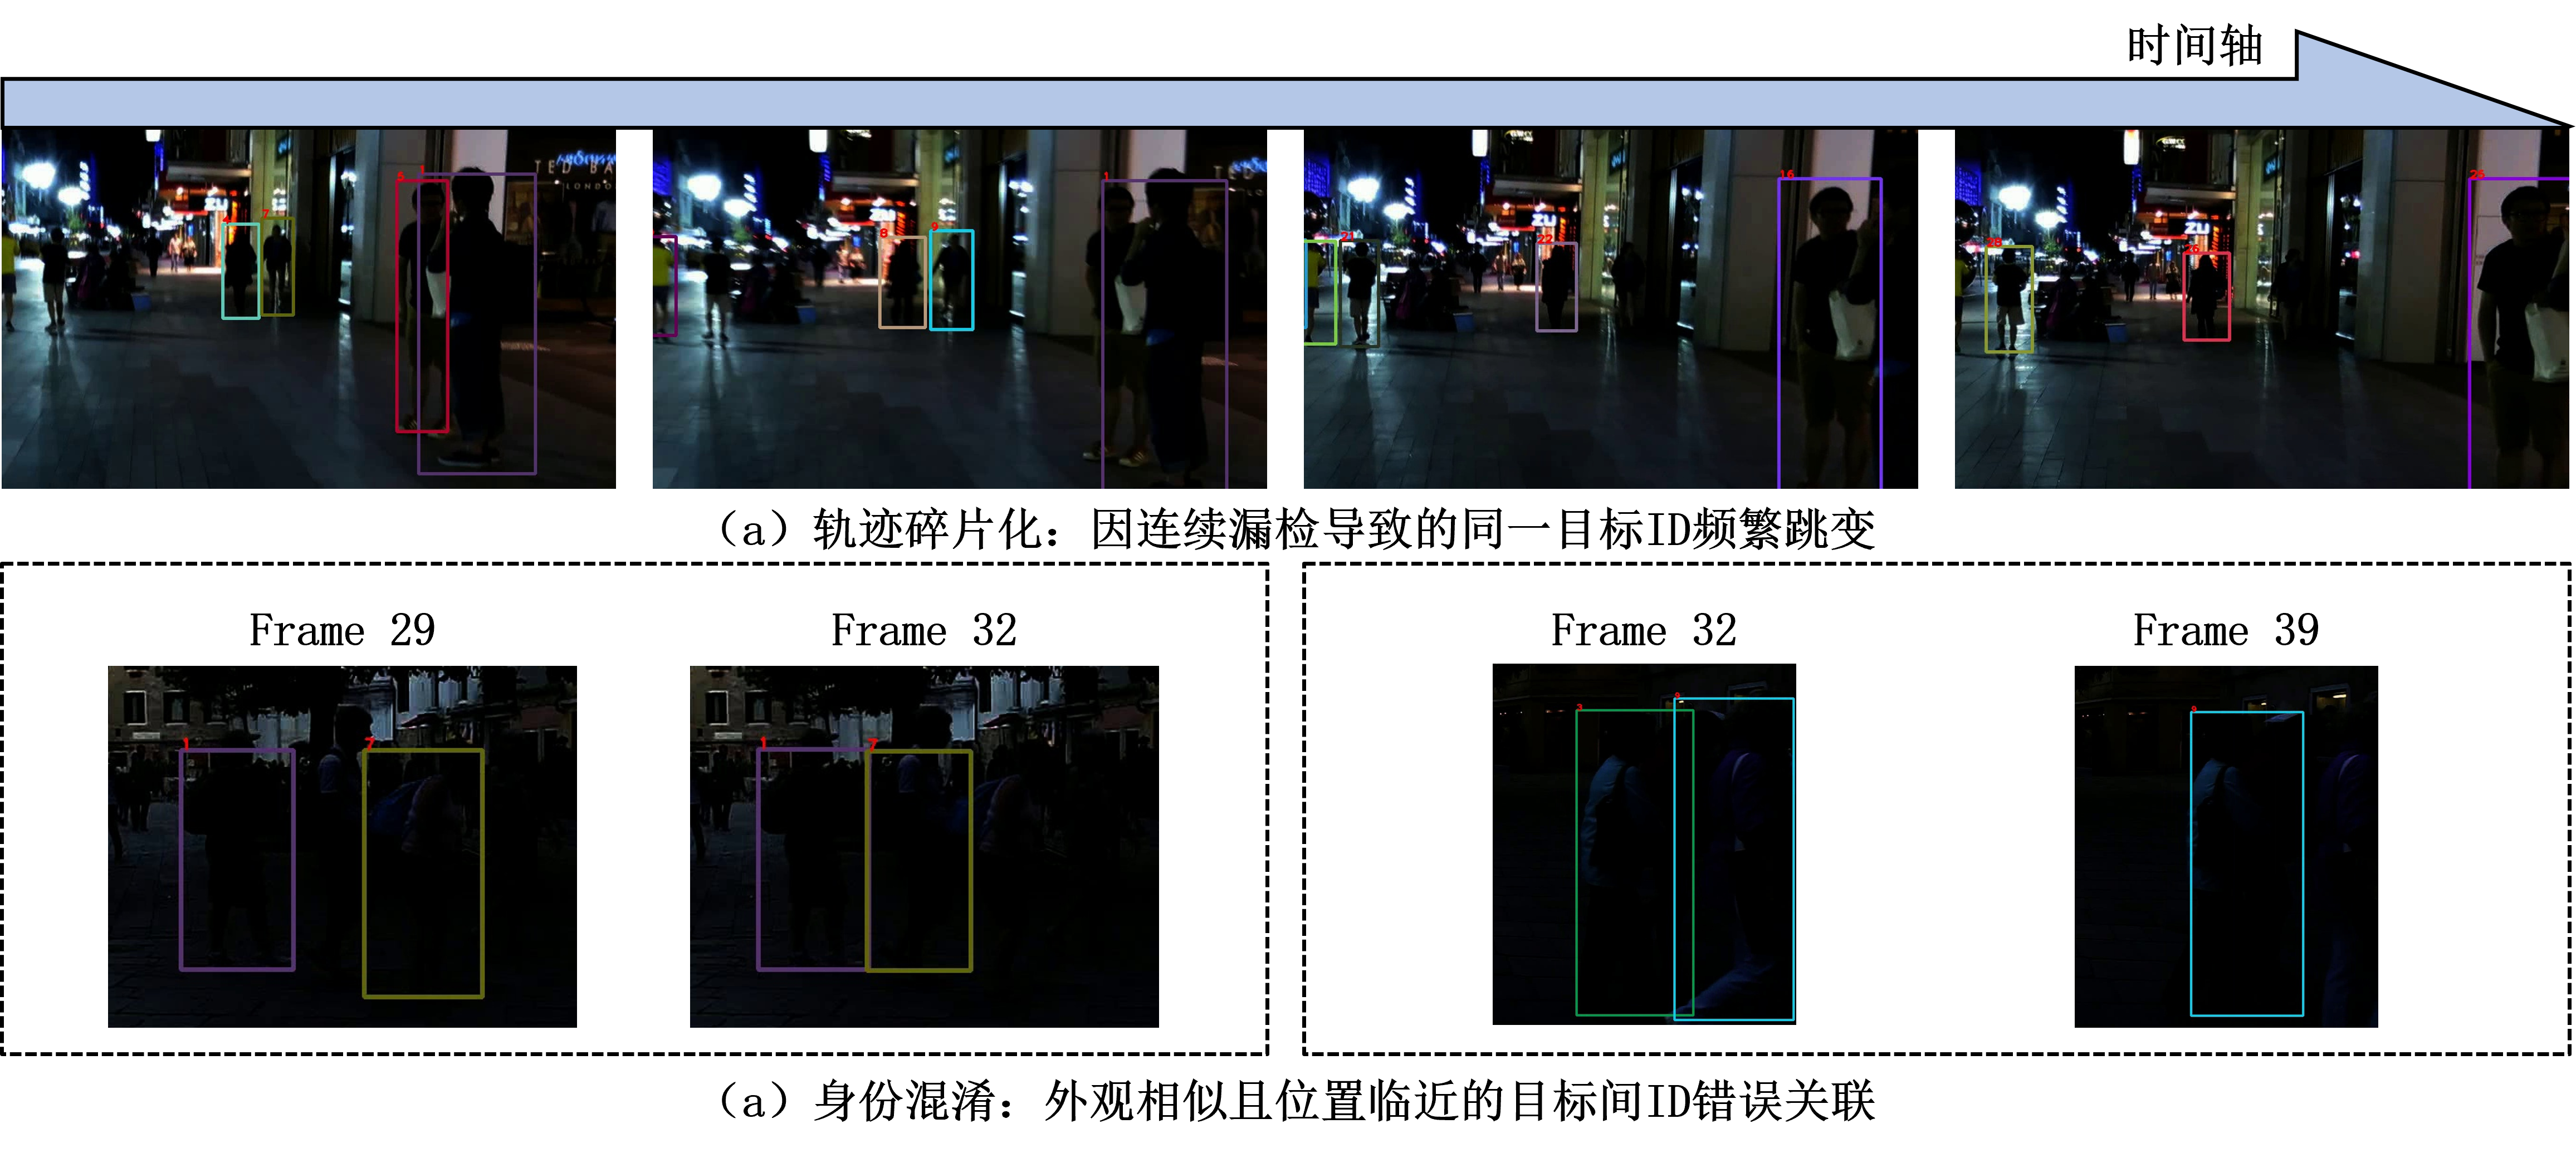
\includegraphics[width=16cm]{chapter3/2.png}
    \caption{\label{fig:ch3_2}DGCTracker整体框架概览}
\end{figure}

如\autoref{fig:ch3_2}所示,DGCTracker的整体工作流程包含三个核心阶段:

\textbf{1. 稀疏图构建}:针对输入的历史轨迹集合$\mathcal{L}^{t-1}$与当前检测集合$\mathcal{D}^{t}$,分别独立构建轨迹图$G^l$与检测图$G^d$。
为了避免全连接带来的计算冗余,本文采用 K-近邻(KNN)算法基于空间欧氏距离自适应生成稀疏拓扑结构;同时,融合目标的外观纹理与几何坐标信息,对图中的节点与边特征进行初始化编码,为后续的消息传递奠定基础。

\textbf{2. 图特征提取}:这是整个框架的核心组成部分。对构建的轨迹图与检测图,并行执行静态图卷积(Static GCN)和动态图卷积(Dynamic GCN)进行特征提取。Static GCN在固定的空间邻域中聚合信息,捕捉目标间稳定的局部几何结构;
Dynamic GCN则基于节点嵌入间的相对差异来动态重构图的连接关系,以显式建模目标间的判别性差异与潜在的长程依赖。最后,通过层次化融合模块,生成多层次上下文信息的判别性节点嵌入。

\textbf{3. 跨帧关联匹配}:基于提取的高维节点嵌入,结合几何重叠度(IOU)先验,计算轨迹与检测之间的亲和度矩阵。最后,通过Sinkhorn\cite{sinkhorn}算法对矩阵进行双随机归一化处理,并利用匈牙利算法\cite{hungarian}完成最终的目标匹配。

为了系统阐述上述方法的具体实现,本节内容安排如下:
\ref{subsec:ch3_2_1} 小节首先详述基于 KNN 的稀疏图构建与特征初始化过程;
\ref{subsec:ch3_2_2} 小节重点介绍双图神经网络的层级化特征提取与融合机制;
\ref{subsec:ch3_2_3} 小节推导跨帧亲和度的计算与可微匹配策略;
最后,\ref{subsec:ch3_2_4} 小节补充介绍提升模型泛化能力的鲁棒性数据增强策略。
\subsection{稀疏图构建}
\label{subsec:ch3_2_1}
为了在降低计算复杂度的同时保留关键的局部空间上下文,本文舍弃了全连接图结构,转而采用基于空间距离的稀疏构图策略。针对历史轨迹集合$\mathcal{L}^{t-1}$与检测集合$\mathcal{D}^{t}$,分别构建轨迹图$G^l=(V^l,E^l)$与检测图$G^d=(V^d,E^d)$。
由于两者的构建过程完全一致,为表述方便,下文统一以轨迹图$G^l$为例进行阐述。

\textbf{1. 基于KNN的拓扑结构建立}

图构建的首要任务是确定节点集合与边集合,即定义图的拓扑结构。将$t-1$时刻的每一个轨迹视为图中的一个节点,形成节点集$V=\{v_i\}_{i=1}^{N_{t-1}}$。类似地,检测图$G^d$的节点集定义为当前时刻的所有检测目标。

在边集合$E^l$的构建上,本文遵循“空间局部性”的假设:即相互靠近的目标之间更可能存在复杂的交互关系(如群体运动、遮挡、碰撞),而距离较远的目标间的影响则相对微弱。若构建全连接图,不仅引入了大量无用的噪声连接,还会导致计算量随节点数量呈平方级增长。

因此,本文采用K-近邻(K-Nearest Neighbors,KNN)算法来动态生成稀疏连接。具体而言,对于图中的任意节点$v_i$,计算其与其他所有节点在图像平面上的欧式距离,并选取距离最近的$k$个邻居节点$\mathcal{N}_k(v_i)$建立有向边:
\begin{equation}
E^l = \{ e_{ji} \mid v_j \in \mathcal{N}_k(v_i),\ \forall\, v_i \in V^l \}
\end{equation}

通过这种策略,图中的每个节点仅与其局部邻域内的$k$个目标(本文默认设置$k=2$)进行交互,将图的规模限制在线性复杂度$\mathcal{O}(kN)$,从而有效地降低了高密度场景下的计算瓶颈,为后续的图卷积操作提供高效的结构基础。

\textbf{2. 节点与边嵌入初始化}

那么在确立了图的拓扑结构之后,我们还需要将目标的外观信息与几何信息映射到图的节点与边上,完成初始嵌入编码,以便图神经网络进行后续的特征挖掘。

\textbf{节点嵌入初始化}:每个节点$v_i$关联两个核心属性:空间位置与外观特征。空间位置由该轨迹在$t-1$时刻的边界框(Bounding Box)表征,包含中心点坐标$(x_i,y_i)$、宽度$w_i$与高度$h_i$。外观特征通过一个预训练好的行人重识别(Person Re-Identification, ReID)网络提取。
该网络以目标的裁剪图像区域为输入,输出一个高维外观特征向量$f_i^{app}\in\mathbb{R}^{2048}$。为了适配图网络的输入维度同时避免特征淹没,进一步引入线性投影层对外观特征进行降维映射,并将其输出作为节点的初始嵌入表示 $h_i^{(0)}\in \mathbb{R}^{32}$。

\textbf{边嵌入初始化}:为了充分利用目标间的空间结构关系,本文将节点间的相对几何差异编码为边特征,作为后续消息传递过程中重要的关系先验。对于一条从源节点$v_j$指向目标节点$v_i$的有向边$e_{ji}$,计算一个包含5个分量的归一化几何向量:
\begin{equation}
\mathbf{g}_{ji} = \left[ \frac{2(x_i-x_j)}{h_i + h_j},\frac{2(y_i-y_j)}{h_i+h_j},\log(\frac{w_i}{w_j}),\log(\frac{h_i}{h_j}),1-\text{DIoU}(i,j) \right]
\end{equation}
其中,几何偏移项$(x_i-x_j)$与$(y_i-y_j)$使用高度进行归一化,主要是考虑到目标高度在多目标跟踪场景中具有较强的时间稳定性与尺度一致性。如在行人等刚性目标中,边界框高度在相邻帧间通常随深度变化而平滑变化,能够
在一定程度上反映目标与摄像机之间的相对距离关系,从而为目标间的空间关系建模提供稳定的参考尺度。中间两项是宽高的对数比值,用于描述相对尺度。最后一项则结合了基于距离的交并比(Distance IoU,DIoU)\cite{DIOU}。相较于传统的IoU,DIoU额外考虑了中心点的归一化距离,能够
更全面地衡量两个框的重叠与对齐程度。

该5维的几何描述子$\mathbf{g}_{ji}$随后喂入一个可学习的非线性投影层$f_\text{MLP}$,映射成16维的边嵌入$z_{ji}^{(0)}\in\mathbb{R}^{16}$:
\begin{equation}
z_{ji}^{(0)} = f_\text{MLP}(\mathbf{g}_{ji})
\end{equation}

至此,稀疏图构建与初始化的完整流程如\autoref{fig:ch3_3}所示。通过上述步骤,原始的检测与轨迹数据被转化为包含稀疏拓扑、节点外观信息及边几何先验的结构化图表示。
这些带有丰富空间上下文信息的图数据,将作为后续图卷积网络的输入,在\ref{subsec:ch3_2_2}节中进行更深层次的特征挖掘与融合。
\begin{figure}[htbp]
    \centering
    \includegraphics[width=16cm]{chapter3/3.png}
    \caption{\label{fig:ch3_3}稀疏图构建与特征初始化流程图}
\end{figure}

\subsection{双图特征提取与层次化融合}
\label{subsec:ch3_2_2}
在上一小节中,我们分别构建了稀疏的轨迹图$G^l$与检测图$G^d$,并完成了节点与边嵌入的初始化。为了后续能够准确度量轨迹与检测之间的亲和度,有必要进一步从图结构中学习同时具备局部几何感知能力与全局语义区分能力的高维节点表示。

鉴于轨迹图与检测图在特征提取阶段采用完全一致的网络结构与参数配置,本节将两者统一抽象为图$G=(V,E)$进行一般化描述,并重点阐述其特征学习机制。

在此统一建模框架下,本文进一步从关系建模的角度出发,将图$G$拆解为静态图$^{s}G$(Static Graph)与动态图$^{d}G$(Dynamic Graph)两种互补表示,分别用于刻画稳定的空间结构关系与判别性的语义差异关系。为了消除概念上的混淆,我们将两者的本质区别定义如下:
\begin{itemize}
    \item \textbf{静态图}$^{s}G$:其拓扑结构由上一小节的基于KNN构建的稀疏邻接关系确定,在特征传播过程中保持不变,以此用于刻画目标在图像平面中的稳定的空间结构关系;
    \item \textbf{动态图}$^{d}G$:与静态图不同的是,其拓扑结构是根据节点嵌入在特征空间中的语义相似性进行动态重构,从而显式挖掘目标之间的判别性关系与潜在的长程依赖。
\end{itemize}

这两种表示分别从空间邻近性和特征相似性这两个正交维度对目标上下文进行建模,形成了互补的特征学习机制。

基于上述定义,我们设计了一个层级递进的双图特征提取与融合模块,整体流程如\autoref{fig:ch3_4}所示。
\begin{figure}[htbp]
    \centering
    \includegraphics[width=16cm]{chapter3/4.png}
    \caption{\label{fig:ch3_4}双图特征提取与层次化融合框架示意图}
\end{figure}

该模块的具体前向传播过程如下:

首先,初始化的图数据被送入静态图卷积分支,利用固定的几何边信息对浅层特征进行局部聚合;

随后,经过静态分支更新的特征被送入动态图卷积(Dynamic GCN)分支,在此处,网络计算节点间的特征相似性并重新构建邻接关系(即重构图结构),进而执行基于语义近邻的消息传递;

上述静态与动态特征更新过程在多个网络层(Layer $\beta$)中递进展开,使得节点表示逐步融合几何结构信息与高层语义信息。

最后,层次化融合模块对各层静态与动态图卷积的输出进行汇集与非线性映射,生成兼顾局部结构一致性与全局语义判别能力的高维节点嵌入表示。

下面将详细阐述这三个核心部件(静态图卷积、动态图卷积及层次化融合模块)的技术细节。

\textbf{1. 静态图卷积(Static Graph Convolution Network,Static GCN)}

静态图卷积旨在利用初始构建的固定拓扑,挖掘目标在物理空间中的局部几何结构特征。在我们的框架中,静态图被定义为$^{s}G=(V,^{s}E)$,其中每个节点的初始嵌入$^{s}h_i\in\mathbb{R}^{32}$源自CNN提取的深度表观特征,
而边嵌入$^{s}z_{ji}\in \mathbb{R}^{16}$则由归一化的相对信息(如距离、宽高、IoU等)建模而成。
\begin{figure}[htbp]
    \centering
    \includegraphics[width=16cm]{chapter3/5.png}
    \caption{\label{fig:ch3_5}静态图卷积(Static GCN)层详细结构}
\end{figure}

受GotFlow3D\cite{GOTFLOW3D}算法启发,为了有效聚合局部邻域内的几何上下文信息,我们设计了如\autoref{fig:ch3_5}所示的Static GCN层。对于第$\beta$层,节点$v_i$的特征更新公式为:
\begin{equation}
    ^{s}h_i^{\beta} = {^{s}g^\beta}\left( ^{s}f_1^\beta\left( ^{s}h_i^{\beta-1} \right) + \max_{j \in \mathcal{N}(i)} {^{s}f_2}^\beta\left( ^{s}z_{ji} ~, \left( ^{s}h_j^{\beta-1} - {^{s}h_i^{\beta-1}} \right) \right) \right)
    \label{equ:sta_gcn}
\end{equation}
其中,$[\cdot]$表示向量拼接操作,$\mathcal{N}_i$为节点$v_i$在静态图中的空间邻居集合(由KNN确定),$^{s}h_i^{\beta-1}$为节点$v_i$在第$\beta-1$层的特征,$^{s}z_{ji}$为从节点$v_j$指向$v_i$的边嵌入。

该公式包含四个核心组件,共同协作以提取局部结构特征:
\begin{itemize}
    \item \textbf{消息函数}$^{s}f_2^\beta (\cdot)$:用于计算邻居节点$v_j$对中心节点$v_i$的消息贡献。其输入为拼接后的向量:边嵌入$^{s}z_{ji}$(编码相对几何关系)与节点特征差$(^{s}h_j^{\beta-1} - {^{s}h_i^{\beta-1}})$(编码局部特征变化模式)。
    最后使用一个多层感知机(MLP)处理此拼接向量,以此来描述邻居$v_j$对目标节点$v_i$的局部结构贡献。
    \item \textbf{聚合函数}$\max$:公式中的$\max$操作用于在邻域$\mathcal{N}_i$内选取响应最强的特征,保留最具判别性的邻居信息,增强模型对遮挡和噪声的鲁棒性。
    \item \textbf{残差层}$^{s}f_1^\beta (\cdot)$:为防止多层图卷积导致的节点特征过平滑(即节点特征趋向同质化),我们引入了跳跃连接。$^{s}f_1^\beta (\cdot)$通常是一个简单的线性变换或浅层MLP,它将节点自身上一层的特征$^{s}h_i^{\beta-1}$映射到与聚合消息相同的特征空间,从而确保节点自身的历史信息得以保留。
    \item \textbf{更新函数}$^{s}g^\beta (\cdot)$:该函数接受残差特征与聚合消息之和,并通过非线性变换输出节点$v_i$在当前层的新特征表示$^{s}h_i^{\beta}$。它决定了如何融合节点自身信息与其局部上下文。
\end{itemize}

为了保证训练的稳定性并提升泛化能力,我们在静态图卷积的每一层可学习组件(包括消息函数 $^{s}f_2^\beta(\cdot)$、跳跃连接层 $^{s}f_1^\beta(\cdot)$ 及更新函数 $^{s}g^\beta(\cdot)$)中均采用GraphNorm\cite{graphnorm}归一化技术。

与计算机视觉中常用的BatchNorm\cite{batchnorm}等归一化方式不同的是,GraphNorm 在归一化时以单个图为单位,
考虑该图内部所有节点的统计信息,而非跨图或跨批次进行归一化。
这一设计对于多目标跟踪任务尤为重要,
因为不同的视频序列(即不同的图)在画面尺寸、目标密度、光照条件等方面存在显著差异,
导致节点与边嵌入的分布各不相同。若使用 BatchNorm,在训练阶段将来自不同图的节点混合进行归一化,
会模糊每个图固有的分布特性,从而损害模型对单个图结构的感知能力。
而 GraphNorm 通过为每个图独立计算归一化统计量,能够更好地保持每个图的全局分布特性,
使模型对不同规模、不同密度、不同场景的图结构都具备良好的适应性和稳定性。此外,GraphNorm 同样也引入了可学习的缩放与偏置参数,以增强特征的表达能力。

最后,通过堆叠$L_s$层静态图卷积,每个节点的有效感受野逐步扩大,能够整合多跳空间邻居的信息。最终,静态图分支输出的特征${^{s}h_i^{L_s}}$编码了以目标自身为中心、由稳定空间邻近关系所定义的局部几何上下文,为后续关联提供了稳健的基础结构先验。

\textbf{2. 动态图卷积(Dynamic Graph Convolution Network,Dynamic GCN)}

静态图卷积基于固定的空间邻域关系(KNN)聚合信息,有效捕获了局部几何结构。
然而,在复杂多变的跟踪场景中,目标间的关联性往往超越简单的空间邻近。例如,在人群密集区域,外观相似同时空间位置接近的目标很容易被错误关联;

考虑到固定空间拓扑的局限性,我们引入了动态图卷积模块。其核心创新在于:
图的邻接关系不再预先固定,而是根据节点在高维特征空间中的语义相似度,在每一层动态重构。
如\autoref{fig:ch3_6}所示,动态图卷积旨在将特征相近的目标显式建模出细粒度的差异信息,从而放大潜在的判别边界,使不同目标在嵌入空间中进一步拉开,以减少后续匹配阶段的混淆。
\begin{figure}[htbp]
    \centering
    \includegraphics[width=16cm]{chapter3/6.png}
    \caption{\label{fig:ch3_6}动态图卷积(Dynamic GCN)层详细结构}
\end{figure}

具体而言,对于第$\beta$层动态图卷积,我们首先基于上一层输出的节点特征$h_i^{\beta-1}$,计算所有节点对在高维特征空间中的余弦距离。对于每一个中心节点$v_i$,我们不再依据空间距离,而是依据余弦距离,选取
与其最相似的$k$个节点作为其动态邻居$\mathcal{N}^{\beta}(i)$。在这一过程中每一层都动态地重建了图的邻接关系,使得网络被强制在特征相近的节点群中寻找具有差异性的维度并加以放大,从而有效推大不同身份节点之间的距离。

定义动态图卷积在第$\beta$层的节点更新公式如下:
\begin{equation}
    ^{d}h_i^{\beta} = \max_{j \in \mathcal{N}^{\beta}(i)} {^{d}f^\beta}\left( \left[^{d}h_{i}^{\beta -1} ~\cdot~\left( ^{d}h_j^{\beta-1} - {^{d}h_i^{\beta-1}} \right) \right] \right)
    \label{equ:dyn_gcn}
\end{equation}
其中,$[\cdot]$表示向量拼接操作,$^{d}f^\beta (\cdot)$为动态图卷积的消息函数。

与静态图卷积不同,动态图卷积并未引入显式的几何边嵌入。
这是因为动态图的邻接关系并非构建于原始图像平面,
而是直接基于节点在高维特征空间中的语义分布动态生成。
在这一设定下,节点之间的关联更多体现在特征表达层面的相似性与差异性,
而非固定的空间约束。
因此,动态图卷积通过显式对比中心节点与其动态邻居在特征维度上的差分信息,
引导网络重点关注语义层面的细粒度差异,
从而更敏锐地捕捉身份判别相关的关键特征。

此外,动态图卷积还具备动态演化的感受野特性。
在静态图卷积中,节点的感受野由其空间 $K$ 近邻所限定,
拓扑结构在整个特征传播过程中保持不变,具有明显的局部性约束。
相比之下,动态图卷积在每一层都会基于更新后的节点特征重新构建邻接关系,
使得节点能够逐层与特征空间中更为相似、但在物理空间上可能相距较远的目标建立联系。
这种自适应、非局部且与语义内容高度相关的感受野演化机制,
使模型能够有效捕获传统局部方法难以建模的高阶依赖关系,
显著增强了特征表示的判别性与鲁棒性。

同样,为保证训练的稳定,动态图卷积中的消息函数 $^{d}f^\beta(\cdot)$ 也采用了 GraphNorm 进行归一化。
通过堆叠 $L_d$ 层动态图卷积,节点特征被不断提纯和增强。
最终,动态图分支输出的特征 ${^{d}h_i^{L_d}}$ 蕴含了丰富的、基于语义相似性的判别信息,
与静态图分支提供的稳健几何结构先验形成有力互补,共同为后续的跨图匹配提供坚实的特征基础。

\textbf{3. 层次化融合模块}

单一视角的特征往往难以全面描述复杂场景下的目标状态。静态图分支输出了包含稳定几何结构的特征序列,而动态图分支则提供了隐含长程语义关联的特征。
为了整合这两类互补的上下文信息,构建一个更加判别且鲁棒的节点表示,我们设计了如\autoref{fig:ch3_7}所示的层次化融合模块。
\begin{figure}[htbp]
    \centering
    \includegraphics[width=16cm]{chapter3/7.png}
    \caption{\label{fig:ch3_7}层次化特征融合模块结构}
\end{figure}

该模块接受来自静态图卷积第$1$至$L_s$层的输出特征${^{s}h_i^1, \dots, ^{s}h_i^{L_s}}$以及动态图卷积第$1$与$L_d$层的输出特征${^{d}h_i^1, \dots, ^{d}h_i^{L_d}}$作为输入。
为了实现各层级多源信息的深度融合,我们定义了如下的聚合与映射机制,来得到最终的节点嵌入$h_G \in \mathbb{R}^{192}$:
\begin{equation}
h_G = \Phi \left( \mathop{\oplus}\limits_{\beta} \left( ^{s}h_i^\beta,~ ^{d}h_i^\beta \right) \right)
\end{equation}
其中,$\oplus_\beta(\cdot)$跨层密集拼接算子,即将所有历史层级的特征向量在通道维度上进行跨图、跨层拼接,形成一个富含多尺度信息的混合特征张量;$\Phi(\cdot)$为带有跳跃连接的一维特征映射函数,
它负责对高维特征进行降维压缩与提纯,在保留原始关键信息的同时,输出紧凑且鲁棒的特征表示。

最终,无论是检测图还是轨迹图,均通过上述双图特征提取与融合模块输出各自的高维节点嵌入,进而用于后续亲和矩阵(Affinity Matrix)的计算,指导更精确的目标关联与匹配。
\subsection{跨帧关联匹配}
\label{subsec:ch3_2_3}
在完成上述特征学习过程后,检测图与轨迹图中的每个节点都获得了高维节点表示。基于此,本小节旨在利用这些具有判别力的节点嵌入,构建跨帧目标之间的亲和矩阵,并通过可微优化算法求解最优
匹配方法,从而完成轨迹的关联与匹配。

\textbf{1. 多模态亲和特征构建}

将轨迹集合中的第$i$个节点与检测集合中的第$j$个节点定义为一个潜在的匹配对,并从以下三个互补维度构建其亲和特征:
\begin{itemize}
    \item \textbf{图节点上下文相似度(Graph Context Similarity)}:基于前述双图特征提取模块输出的高维节点嵌入$h_i^l$与$h_j^d$,计算两者的余弦相似度。该特征聚合了多阶邻域信息,反映了目标对的高维语义与拓扑结构上的一致性。
    \item \textbf{表观纹理相似度(Appearance Texture Similarity)}:我们复用\ref{subsec:ch3_2_1}小节中定义的初始节点嵌入$h^{l,(0)}$与$h^{d,(0)}$,即由ReID骨干网络降维投影后的表观特征,并计算目标对的表观相似度。该特征能够捕捉目标最原始的视觉纹理色彩信息,弥补图卷积过程中可能平滑掉的个体细节。
    \item \textbf{几何运动一致性(Geometric Consistency)}:为了缓解行人姿态变化导致的包围框宽度不稳定性,本文采用高度感知交并比(HIoU) 。HIoU 仅基于高度方向计算重叠率,从而将几何约束重点聚焦于目标的深度一致性,有效剔除物理空间上不合理的候选匹配,提升了关联层对遮挡和形变的鲁棒性。
\end{itemize}

为了自适应地融合上述异构信息,我们将三种相似度矩阵在通道维度上进行拼接,构建出一个三维的粗粒度亲和张量。随后,将其送入一个由多层感知机(MLP)构成的亲和预测层(Affinity Layer)。该层通过学习不同模态在关联决策中的权重,并经过Sigmoid激活函数映射,输出最终的亲和得分。

整个多模态融合与打分过程可统一表述为:
\begin{equation}
S_{ij} = \sigma \left( \mathcal{M} \left( \left[
\underbrace{\cos(h^l_i, h^d_j)}_{\text{Graph Context}}, ~
\underbrace{\cos(h_i^{l,(0)}, h_j^{d,(0)})}_{\text{Appearance}}, ~
\underbrace{\text{HIoU}(b^l_i, b^d_j)}_{\text{Geometric}}
\right] \right) \right)
\end{equation}
其中,$[\cdot]$表示向量拼接操作,$\cos(\cdot,\cdot)$为余弦相似性度量,$\mathcal{M}(\cdot)$为多层感知机,$\sigma (\cdot)$为Sigmoid激活函数;$b_i^l$与$b_j^d$分别代表轨迹包围框与检测框,最终得到的$S_{ij}\in (0,1)$即为轨迹$i$与检测$j$的亲和分数,数值越高代表两者为同一个目标的可能性越大。

\textbf{2. 基于Sinkhorn的可微关联优化}

在前一阶段,我们明确了单个匹配对的亲和分数$s_{ij}$的计算方式。进一步地,从矩阵建模角度看,所有轨迹$\mathcal{L}=\{l_i^{t-1}\}_{i=1}^{N}$与检测$\mathcal{D} = \{d_j^t\}_{j=1}^{M}$之间的关联关系可统一表示为亲和矩阵 $ S \in \mathbb{R}^{N \times M}$。
回顾\ref{sec:ch3_1}中对在线跟踪任务的建模,我们需要进一步在亲和矩阵$S$的基础上求解互斥约束下的最优匹配问题,使得每条轨迹至多匹配一个检测,同时每个检测也至多分配给一条轨迹。

然而,在实际跟踪场景中经常会存在目标新生(当前帧出现新目标)与轨迹消亡(现有目标离开视野)等情况,因此我们引入广义轨迹节点与广义检测节点,对原始亲和矩阵$S$进行增广,构造增广亲和矩阵$\overline{S}\in \mathbb{R}^{(N+1) \times (M+1)}$。具体而言,
我们在$S$的右侧添加一列,对应一个广义检测节点,用于吸收未匹配的轨迹(即轨迹消亡的可能性);在$S$的底部添加一行,对应一个广义轨迹节点,用于吸收未匹配的检测(即目标新生的可能性)。新增的行与列元素值由一个可学习参数$\alpha\in \mathbb{R}$填充:
\begin{equation}
\overline{S}_{ij} = 
\left\{
    \begin{array}{ll}
        S_{ij}, & \text{if } i \in \{1, \dots, N\} \text{ and } j \in \{1, \dots, M\} \\
        \alpha, & \text{if } i = N+1 \text{ or } j = M+1
    \end{array}
\right.
\end{equation}
其中$\alpha$在训练过程中被优化,其值反映了模型对目标出现或消失的先验置信度。

为了确保全局匹配的合法性,增广后的亲和矩阵$\overline{S}$需满足如下新的边缘分布约束:
\begin{equation}
\overline{S} \, \mathbf{1}_{M+1} = \begin{bmatrix} \mathbf{1}_N^\top, & M \end{bmatrix}^\top \quad \text{and} \quad \overline{S}^\top \, \mathbf{1}_{N+1} = \begin{bmatrix} \mathbf{1}_M^\top, & N \end{bmatrix}^\top
\label{equ:constraint}
\end{equation}
其中,$\mathbf{1}_k$表示维度为$k$的全1向量。该约束的物理含义为对于前 $N$ 行(真实轨迹),
其亲和度之和应为 $1$,表示每条轨迹要么匹配到一个检测,要么被视为“消亡”并被广义检测节点吸收;
对于前 $M$ 列(真实检测),其亲和度之和也应为 $1$,表示每个检测要么匹配到一条轨迹,要么被视为“新生”并被广义轨迹节点吸收。
新增的广义节点对应的行(列)和分别等于 $M$ 和 $N$,以平衡整个关联系统中的流量守恒。

为求解满足上述边际约束的亲和矩阵,我们采用Sinkhorn算法\cite{sinkhorn}对增广矩阵$\overline{S}$进行优化求解。

Sinkhorn 算法最初用于求解带有边缘分布约束的最优传输问题,其核心思想是通过对矩阵行与列进行交替归一化操作,使矩阵逐步逼近满足给定边缘分布的双随机矩阵(Doubly Stochastic Matrix)。
与传统匈牙利算法直接求解离散最优匹配不同,Sinkhorn 算法的迭代过程是连续且可微的,因此可作为匈牙利算法的一种可微松弛形式,被广泛应用于深度学习框架中的软指派(soft assignment)问题。

具体迭代步骤如下:设初始增广矩阵为 $\overline{S}^{(0)} = \overline{S}$,设定目标行和向量$\mathbf{r}$和目标列向量$\mathbf{c}$分别为:
\begin{equation}
    \begin{dcases}
        \mathbf{r} = [\underbrace{1,\dots,1}_{N}, M]^\top \\
        \mathbf{c} = [\underbrace{1,\dots,1}_{M}, N]^\top
    \end{dcases}
\end{equation}
在第 $k$ 次迭代中($k=1,\dots,T$),交替执行以下两步归一化操作:

\textbf{Step 1. 行归一化(Row Normalization)}:首先计算当前矩阵 $\overline{S}^{(k-1)}$ 的行和,利用目标行和向量 $\mathbf{r}$ 对矩阵的每一行进行缩放,使其满足行边缘约束:
\begin{equation}
    U^{(k)} = \text{diag}\left( \mathbf{r} \oslash \left( \overline{S}^{(k-1)} \mathbf{1}_{M+1} \right) \right) \overline{S}^{(k-1)}
\end{equation}
其中,$\oslash$ 表示逐元素除法,$\mathbf{1}_{d}$ 为 $d$ 维全1列向量,$\text{diag}(\cdot)$ 表示以向量元素构建对角矩阵。

\textbf{Step 2. 列归一化(Column Normalization)}:基于行归一化后的中间矩阵 $U^{(k)}$,计算其列和,并利用目标列和向量 $\mathbf{c}$ 对矩阵的每一列进行缩放,使其满足列边缘约束:
\begin{equation}
    \overline{S}^{(k)} = U^{(k)} \text{diag}\left( \mathbf{c} \oslash \left( (U^{(k)})^\top \mathbf{1}_{N+1} \right) \right)
\end{equation}

交替执行以上 $T$ 次迭代后,得到优化后的矩阵 $\overline{S}^{(T)}$,此时矩阵的行和与列和已收敛至目标向量 $\mathbf{r}$ 与 $\mathbf{c}$,从而逐步逼近并满足\autoref{equ:constraint}中定义的边际约束。

最终,为了获取针对原始轨迹集与检测集的关联结果,我们对收敛后的增广矩阵$\overline{S}$执行裁剪操作,即去除辅助的广义行与广义列,得到最终的优化亲和矩阵$\hat{S}\in \mathbb{R}^{N\times M}$。
\begin{equation}
\hat{S} = \overline{S}^{(T)}_{1:N, 1:M} 
\end{equation}
此时,矩阵 $\hat{S}$ 中的元素 $\hat{S}_{ij}$ 表示在满足互斥约束的条件下,
轨迹 $l_i^{t-1}$ 与检测 $d_j^{t}$ 之间的软匹配权重,该权重可视为原始亲和分数在全局约束下的归一化结果,
并在训练阶段作为匹配概率的连续松弛形式参与损失计算。

上述基于Sinkhorn的可微关联优化过程,在保证一对一匹配约束的同时,实现了从亲和矩阵到软指派结果的连续映射,为后续的损失函数设计与在线推理阶段的离散匹配提供了统一的优化基础。

\textbf{3. 损失函数与推理决策}

\textbf{(1) 训练阶段}

在训练阶段,我们将经Sinkhorn优化后的亲和矩阵$\hat{S}$作为监督对象。设$Y\in\{0,1\}^{N\times M}$为轨迹-检测的真实匹配标签矩阵,其中$Y_{ij}=1$表示轨迹$l_i^{t-1}$与检测$d_j^{t}$属于同一目标,否则$Y_{ij}=0$。

由于在线多目标跟踪中正负样本比例严重失衡(绝大多数轨迹-检测对为负样本),若直接采用标准二元交叉熵容易导致训练被大量易分类负样本主导,
从而削弱了模型对困难样本(易混淆匹配)的学习能力。
为此,本文采用 Focal Loss \cite{focalloss}对亲和矩阵进行监督学习,
以增强模型对难分类样本的关注。

首先定义逐元素的分类置信度矩阵$p_t$:
\begin{equation}
p_t = Y\odot \hat{S} + (1 -Y) \odot (1 - \hat{S})
\end{equation}
其中,$\odot$表示逐元素乘积。当$Y_{ij}=1$时,$p_t=\hat{S}_{ij}$;当$Y_{ij}=0$时,$p_t=1-\hat{S}_{ij}$。

基于此,关联损失函数定义为:
\begin{equation}
    L_{\mathrm{assoc}} = -\frac{1}{B} \sum_{b=1}^B
    \left[
        \alpha (1 - p_t)^{\gamma} \odot \Bigl( Y \odot \log(\hat{S}) + (1 - Y) \odot \log(1 - \hat{S}) \Bigr)
    \right]
    \label{equ:gnn_loss}
\end{equation}
其中$B$表示一个批次中参与训练的图样本数量,$\alpha \in (0,1)$为正样本权重系数,用于平衡正负样本贡献,$\gamma \ge 0$为调制因子,用于抑制易分类样本对整体损失的影响。
    
通过最小化上述损失函数,模型能够在端到端训练过程中学习到更加鲁棒的跨帧关联评分,从而提升复杂场景下目标匹配准确性与身份一致性。
    
\textbf{(2) 推理阶段}

在推理阶段,为获得满足严格互斥约束的一对一离散匹配结果,本文将$\hat{S}$转换为代价矩阵并采用匈牙利算法求解最优二分匹配。具体地,可定义代价为:
\begin{equation}
    C=1-\hat{S}
\end{equation}

然后,再通过匈牙利算法得到离散指派矩阵$A\in\{0,1\}^{N\times M}$,其中$A_{ij}=1$表示轨迹$l_i^{t-1}$与检测$d_j^{t}$被匹配。
需要指出的是,本节所描述的关联过程仅针对相邻两帧之间的匹配决策,用于刻画轨迹与检测在当前时刻$t$的局部对应关系。
未匹配目标在更长时间尺度上的状态演化与轨迹维护策略,将在\ref{sec:ch3_3}节中结合完整的轨迹管理机制进行统一说明。

综上所述,DGCTracker 在训练阶段通过可微 Sinkhorn 层实现端到端优化,在推理阶段结合匈牙利算法保证物理约束的严格性,从而实现了跨帧目标的高精度稳定跟踪。

\subsection{鲁棒性数据增强策略}
\label{subsec:ch3_2_4}

本章提出的DGCTracker依赖于高质量的图结构来进行关系推理。在理想情况下,相邻帧的轨迹图与检测图在拓扑结构上应具有高度的相似性。然而,在实际的跟踪场景中,视频序列常存在
帧率波动、相机运动、检测器漏检或定位偏差等问题,导致输入模型的图数据往往是不完备且含有噪声的。为提升DGCTracker在动态、不完备数据条件下的泛化能力与鲁棒性,我们设计了三种
针对图结构的在线数据增强策略(如\autoref{fig:ch3_8}所示):
\begin{figure}[htbp]
    \centering
    \includegraphics[width=16cm]{chapter3/8.png}
    \caption{\label{fig:ch3_8}鲁棒性数据增强策略示意图}
\end{figure}

\textbf{1. 随机帧间隔采样(Random Frame Interval Sampling)}

在线跟踪算法通常假设相邻帧间目标运动平滑、外观变化微小。然而,低视频帧率或相机快速移动会破坏这一假设,导致目标在相邻帧间产生较大位移,增大关联难度。

为增强模型对时序间隔变化的适应性,我们采用随机帧间隔采样策略。具体而言,在训练阶段,我们不再固定使用相邻两帧$(t-1, t)$构建样本,
而是以概率$p_{\mathrm{interval}}$从当前帧$t$的历史帧窗口$[t-\Delta_{\max}, t-1]$中随机采样一帧$t'$作为"历史帧"。
其中,$\Delta_{\max}$为预设的最大回溯间隔(如$\Delta_{\max}=5$)。此时,轨迹图$G^l$基于$t'$时刻的真实轨迹构建,而检测图$G^d$基于$t$时刻的检测构建。

此策略通过人为引入随机的、非连续的时序间隔,有效模拟了低帧率视频与相机抖动带来的挑战。它迫使模型不仅依赖短时运动平滑性先验,更需要从外观特征和更复杂的空间布局关系中寻找关联依据,从而提升了对运动突变场景的鲁棒性。

\textbf{2. 随机节点失活(Random Node Inactivation)}

目标检测器在实际应用中难以保证百分之百的召回率,漏检(Missed Detection)是导致轨迹中断的主要因素之一。为增强模型对不完备图结构的适应能力,我们引入了随机节点失活策略。

在每次训练迭代中,对于构建好的轨迹图$G^l$和检测图$G^d$,我们以独立的概率$p_{\mathrm{inactivate}}$随机“丢弃”图中的一部分节点及其所有关联边。具体实现中,被选中的节点特征向量将被置为零向量,同时其对应的边也从邻接表中移除。

这一操作直接模拟了检测器漏检或目标短暂消失(如被完全遮挡)的情形。它迫使图神经网络必须在一个拓扑结构不完整、信息缺失的图上进行消息传递与特征聚合,从而学习到在节点缺失情况下仍能保持有效推理的能力,降低了模型对“全图”结构的过拟合,提升了在面对真实检测噪声时的稳定性。

\textbf{3. 随机几何噪声注入(Random Geometric Noise Injection)}

检测器提供的边界框(Bounding Box)通常包含一定的定位误差,其中心点坐标与宽高尺寸并非绝对精确。为了增强模型对几何输入噪声的鲁棒性,并使学习到的特征表示对微小形变不敏感,我们设计了随机几何噪声注入策略,
即在训练阶段对轨迹和检测框的几何属性(中心点坐标、宽高)注入服从高斯分布的随机扰动:
\begin{equation}
    b'_{x,y,w,h} = b_{x,y,w,h} + \mathcal{N}(0, \sigma^2_{geo})
\end{equation}

该策略通过扰动节点的空间位置与尺度信息,模拟了实际检测框的定位抖动与尺度估计误差。它促使模型在构建边嵌入(依赖相对几何信息)和计算几何相似度(如HIoU)时,不过度依赖于精确的坐标值,从而学习到对几何噪声更具容错性的特征表示与关联度量。

上述三种增强策略以一定的概率组合应用。他们的协同作用,从时序连续性、数据完备性和空间精确性三个不同维度构造了多样化的训练样本分布。
通过在这种“增强后”的、更接近真实世界复杂性的数据上进行端到端优化,DGCTracker 能够学习到更加稳健的特征提取器与关联推理机制,从而在面对实际视频流中各种不确定因素时,表现出更强的泛化能力和跟踪稳定性。
消融实验(见表 \ref{tab:ch_3_4_3_10})结果证实,引入这些数据增强策略后,模型在 MOT17 基准上的 HOTA、IDF1 和 MOTA 指标均获得显著提升,验证了其有效性。

\section{轨迹状态管理策略}
\label{sec:ch3_3}
对于在线多目标跟踪任务来说,轨迹的生成、维持与终止是一个随时间动态演化的过程。仅依赖单帧或局部匹配结果进行轨迹更新,容易受到检测误差、短时遮挡以及误检噪声的干扰,从而导致轨迹碎片化或身份切换问题。
因此,在跨帧关联结果的基础上,引入合理的轨迹状态管理机制,对轨迹在时间维度上的行为进行建模,是保证跟踪系统稳定性与鲁棒性的关键。

本节提出的轨迹状态管理策略,在整体设计上参考了ByteTrack\cite{bytetrack}的基本框架,并与\ref{subsec:ch3_2_3}节提出的基于图神经网络的关联结构深度融合。
通过显式建模轨迹的生命周期状态,结合三阶段级联匹配策略完成状态迁移与轨迹更新,在保证跟踪精度的同时,实现对检测噪声抑制、目标遮挡恢复及身份一致性保持的综合优化。
\subsection{轨迹生命周期建模}
为了准确描述目标在视频序列中的时空演化过程,我们将轨迹$\mathcal{L}$的生命周期划分为四种互斥状态:新生(Born)、活跃(Active)、休眠(Sleep)和消亡(Dead)。各状态的物理含义及状态转移逻辑(如图 \ref{fig:state_machine} 所示)定义如下:
\begin{figure}[htbp]
    \centering
    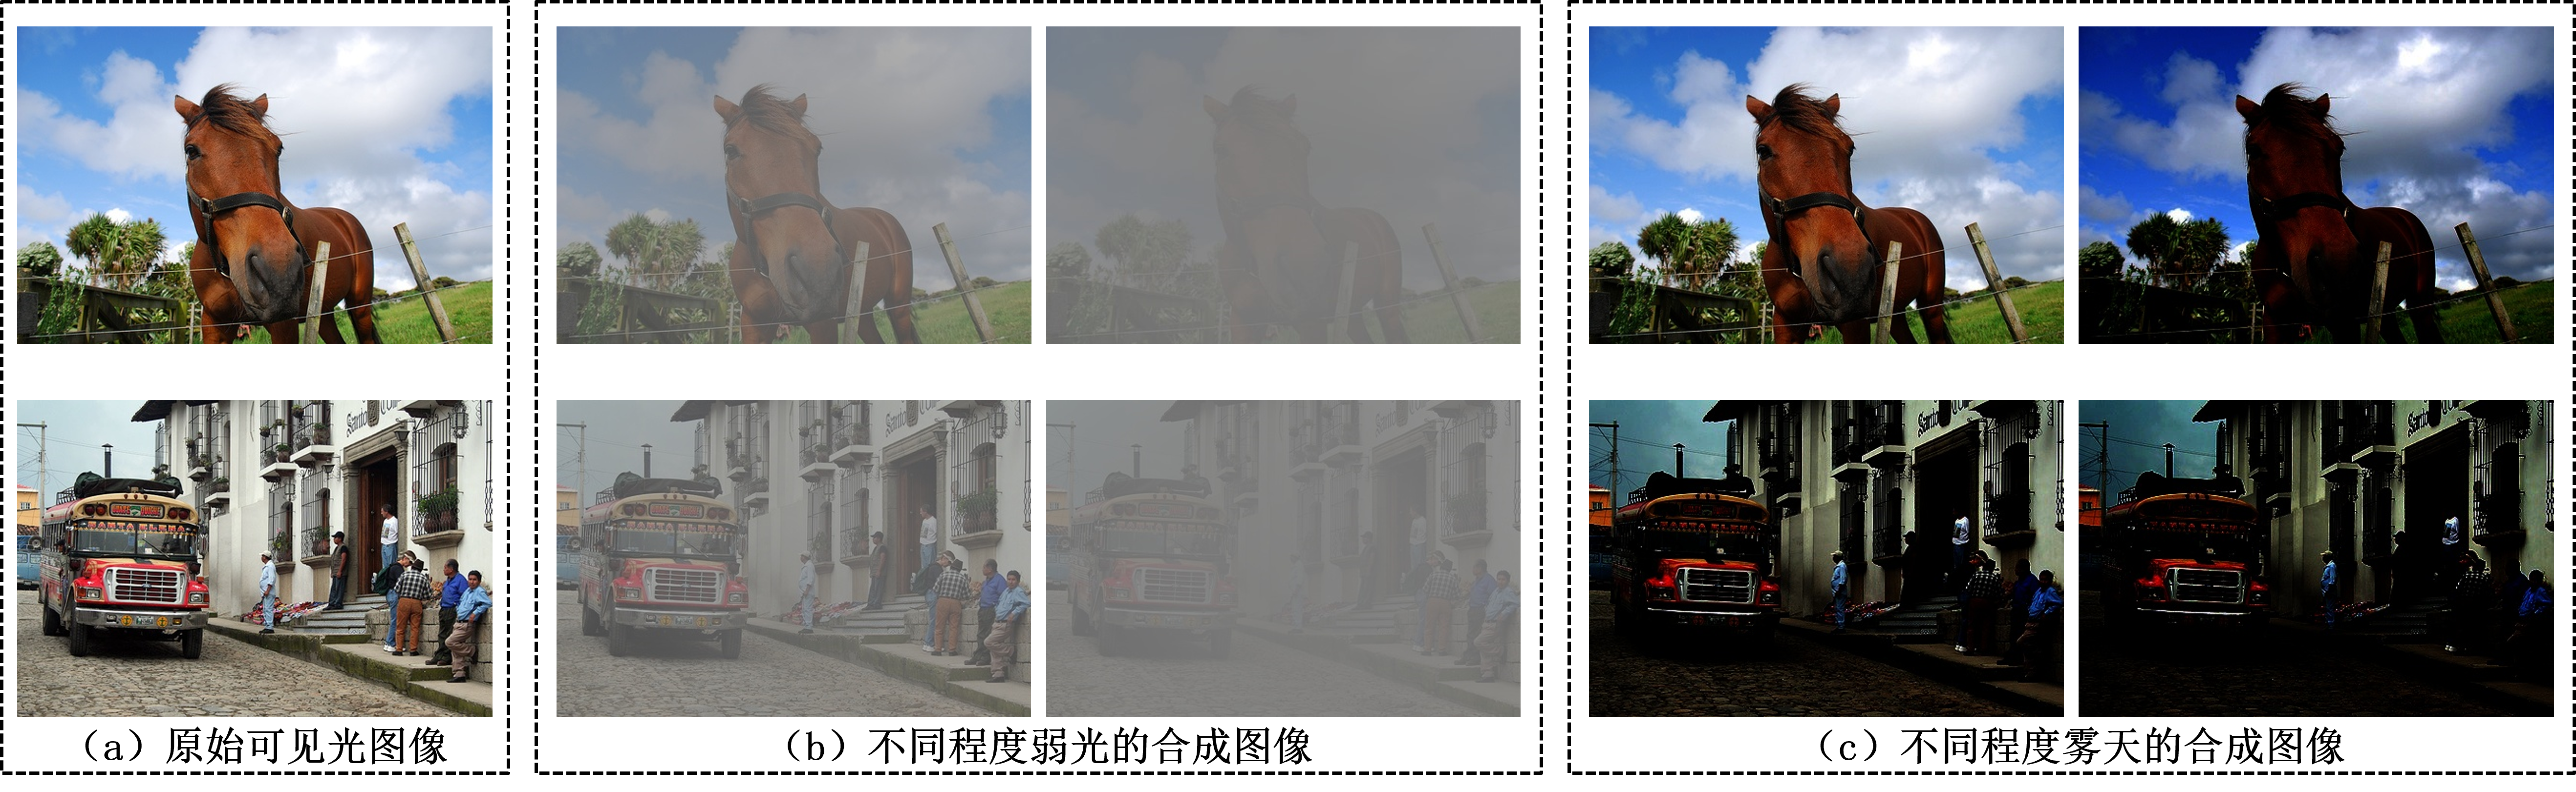
\includegraphics[width=16cm]{chapter3/9.png}
    \caption{\label{fig:state_machine}轨迹生命周期四状态转移示意图}
\end{figure}

\begin{itemize}
    \item \textbf{新生状态(Born)}:表示由当前帧检测结果初始化的潜在目标候选。由于检测器可能会将背景误检为目标(False Positive),为了抑制检测噪声,所有由高置信度检测框初始化但尚未通过时间连续性验证的轨迹均被标记为 Born 状态。该状态下的轨迹暂不参与身份分配与结果输出。
    具体而言,若 Born 状态轨迹在随后的 $N_{\text{init}}$ 帧内(默认设置为 3 帧)能够持续匹配到高置信度检测结果,则认为该目标具有较高的真实性,其状态升级为 Active;否则,该轨迹被判定为噪声并直接转移至 Dead 状态。

    \item \textbf{活跃状态(Active)}:表示当前视野内已被系统确认存在的跟踪目标。只有处于 Active 状态的轨迹才会被分配唯一的全局身份标识(ID),并作为最终跟踪结果对外输出。当轨迹在当前帧成功完成关联时,系统将利用最新观测对其状态进行更新;若匹配失败(例如发生短时遮挡或检测漏失),
则轨迹转入 Sleep 状态以保留其历史信息。

    \item \textbf{休眠状态(Sleep)}:用于刻画目标因短期遮挡、运动模糊或检测失败而暂时不可观测的情形,亦可视为轨迹的“丢失(Lost)”状态。系统将为处于该状态的轨迹保留其最近一次有效观测信息,并在后续帧中持续尝试重新关联。若在最大保留时间 $T_{\max}$ 内(默认设置为 30 帧)重新匹配成功,
    轨迹状态将被恢复为 Active;否则,认为目标已彻底离开视野,其状态转移至 Dead。

    \item \textbf{消亡状态(Dead)}:表示目标已彻底消失或被判定为噪声。该状态为终止状态,系统将释放其内存资源,不再参与后续计算。
\end{itemize}

\subsection{三阶段轨迹管理策略}
基于上述生命周期模型,我们进一步设计了一种三阶段级联的轨迹管理策略,用于在不同可靠性层级下逐步完成轨迹与检测之间的匹配,并据此实现轨迹状态迁移与维护。
该策略以高置信关联结果优先、低置信匹配逐级补充为基本原则,通过多层次约束逐步筛选有效关联关系,在保证匹配精度的同时有效抑制检测噪声的干扰。

其完整执行流程如\autoref{fig:track_management}所示,算法伪代码详见附录\ref{sec:track_management}。
具体而言,在每一时间步 $t$,系统按以下流程执行:
\begin{figure}[htbp]
    \centering
    \includegraphics[width=13cm]{chapter3/10.png}
    \caption{\label{fig:track_management}DGCTracker三阶段轨迹管理流程图}
\end{figure}

\textbf{1. 数据预处理}

首先,根据预设的检测置信度阈值$\tau$(默认为 0.6),将当前帧的检测框集合$\mathcal{D}^t$划分为高置信度子集$D_{high}$与低置信度子集$D_{low}$:
\begin{equation}
\begin{dcases}
D_{\text{high}} = \{\, d \in \mathcal{D}^t \mid d.\text{score} \ge \tau \,\},\\
D_{\text{low}}  = \{\, d \in \mathcal{D}^t \mid d.\text{score} < \tau \,\}.
\end{dcases}
\end{equation}

同时,将上一帧的轨迹集合$\mathcal{L}^{t-1}$,按其状态划分成三个子集:
\begin{equation}
\begin{dcases}
L_{\text{born}} = \{\, l \in \mathcal{L}^{t-1} \mid l.\text{state} = \mathbf{BORN} \,\},\\
L_{\text{active}}  = \{\, l \in \mathcal{L}^{t-1} \mid l.\text{state} = \mathbf{ACTIVE} \,\}, \\
L_{\text{sleep}}  = \{\, l \in \mathcal{L}^{t-1} \mid l.\text{state}  = \mathbf{SLEEP} \,\}. 
\end{dcases}
\end{equation}
其中,消亡(DEAD)状态的轨迹已被系统移除,不参与后续计算。

\textbf{2. 三阶段级联匹配}

匹配过程按优先级从高到低依次执行,前一阶段的未匹配结果将传递至后续阶段作为输入。

\textbf{阶段一:基于图关联的主匹配阶段}

本阶段旨在实现高可见度、高置信度目标的精确关联。将活跃轨迹集$L_{\text{active}}$与高置信度检测框$D_{\text{high}}$分别构建为轨迹图与检测图,并利用本文核心方法——双图协同关联网络(DGC)计算二者间的亲和度矩阵$\hat{S}$:
\begin{equation}
    \hat{S} = \text{DGC}(L_\text{active},D_\text{high})
\end{equation}

矩阵$\hat{S}$综合了基于图上下文的高级语义相似性、原始外观特征相似性以及改进的几何相似性(HIoU)。
随后,采用匈牙利算法对$\hat{S}$进行优化求解,得到最优匹配对集合$match_1$。
匹配成功的活跃轨迹将维持其状态并更新运动与外观模型;未匹配的活跃轨迹$L_{\text{remain}}$与未匹配的高置信度检测框$D_{\text{remain}}$将流入下一阶段。

\textbf{阶段二:多模态联合匹配阶段}

本阶段旨在恢复因短暂遮挡或运动模糊而丢失的目标。将阶段一未匹配的活跃轨迹$L_{\text{remain}}$与所有休眠轨迹$L_{\text{sleep}}$合并,构成候选轨迹集$L_2 = L_{\text{remain}} \cup L_{\text{sleep}}$。
随后,计算$L_2$与低置信度检测框$D_{\text{low}}^t$之间的匹配代价矩阵$C$:
\begin{equation}
    C_{i,j} = (1-\lambda) \cdot C_{\text{app}}(d_i,l_j)  + \lambda\cdot C_{\text{HIoU}}(d_i,l_j)
\end{equation}
其中,$C_{\text{app}}$为外观特征的余弦距离,$C_{\text{HIoU}}$为考虑中心点距离的改进交并比度量,超参数$\lambda$用于平衡两项的权重。
此设计允许系统在目标外观可能退化时,更依赖稳健的几何信息进行关联。同样通过匈牙利算法求解得到匹配对$match_2$。

\textbf{阶段三:基于 IoU 的新生轨迹验证阶段}

经过前两轮筛选,我们利用剩余的高分检测框 $D_{\text{remain}}$ 对待确认的新生轨迹 $L_{\text{born}}$ 进行验证。
由于新生轨迹尚未建立稳定的外观模型,且通常没有复杂的运动历史,我们采用计算高效的交并比(IoU)代价矩阵进行几何匹配。匈牙利算法将基于此代价矩阵求解最优匹配对 $match_3$。

\textbf{3. 状态维护与更新}

整合三个阶段的所有匹配结果$match = match_1 \cup match_2 \cup match_3$后,系统按以下规则更新轨迹状态:
\begin{itemize}
    \item \textbf{匹配成功的轨迹}:若为Active或Sleep轨迹,则更新其状态为Active;若为Born轨迹,则其连续匹配成功计数器加1,当计数器达到阈值$N_{\text{init}}$(默认3)时,转为Active状态并分配全局唯一ID。
    \item \textbf{未匹配的轨迹}:Active轨迹转为Sleep状态;Sleep轨迹的丢失帧数加1,若超过最大保留时长$T_{\text{max}}$(默认30帧),则转为Dead状态;Born轨迹直接转为Dead状态,视为噪声滤除。
\end{itemize}

最终,系统输出更新后的轨迹集合$L^t$,完成当前帧的跟踪。该三阶段级联策略通过精细化、分优先级的资源分配,在确保高精度关联的基础上,显著提升了系统对复杂场景的适应性与轨迹的长期一致性。

\section{实验结果与讨论}
\label{sec:ch3_4}
为了全面验证本章提出的基于图神经网络的轨迹关联方法(DGCTracker)的有效性,我们在公开多目标跟踪基准数据集上进行了广泛的实验验证与分析。
本节内容安排如下:
首先,\ref{subsec:ch3_4_1} 节详细阐述了实验的基础设置,包括数据集的本地划分策略、采用的各项评价指标体系以及模型训练的实现细节;
其次,\ref{subsec:ch3_4_2} 节将本方法与当前主流的先进算法(State-of-the-Arts)进行对比,从客观指标和主观可视化两个维度评估算法的综合性能;
最后,\ref{subsec:ch3_4_3} 节通过一系列消融实验,深入剖析了稀疏图构建参数、双图神经网络架构以及数据增强策略对模型最终跟踪精度的具体影响与贡献。
\subsection{实验条件设置}
\label{subsec:ch3_4_1}
\textbf{1. 数据集与评价指标}

我们选用 MOT Challenge 系列数据集作为主要评测基准。其中,对比实验在 MOT16 和 MOT17 数据集上进行,旨在将所提出的 DGCTracker 方法与当前主流的先进跟踪算法(包括基于图的方法及经典的 SORT 系列方法等)进行横向对比;
消融实验则统一基于 MOT17 数据集展开,以保证不同模块配置下实验结果的可比性。

由于官方 MOT Challenge 评估服务器访问受限,为进行有效的消融研究与性能对比,我们采用一种在学术研究中广泛使用的替代划分方案。具体而言,对于 MOT16 与 MOT17 的每一个训练视频序列,我们将其最后连续的100帧划出作为测试集,其余帧则作为训练集。
本节的所有定量实验均在此测试集上报告,以确保评估环境的一致性与公平性。

此外,为了公平地评估本文提出的关联算法性能,并排除检测器质量差异带来的干扰,本节所有实验均严格遵循 Public Detection(公共检测)协议,即直接使用数据集官方提供的检测结果,而不引入额外的私有检测器进行推理。具体而言,在 MOT16 上使用 DPM 检测器结果,在 MOT17 上使用 SDP 检测器结果。

在性能评估方面,我们采用多目标跟踪领域权威的评估工具包TrackEval\cite{TrackEval_2020}进行量化评估。使用的核心评价指标如第\ref{subsec:ch2_3_1}节所述,
包括:高阶跟踪精度(HOTA)、检测精度(DetA)、关联精度(AssA)、识别F1分数(IDF1)、身份精确率(IDP)、身份召回率(IDR)、多目标跟踪精度(MOTA)和多目标跟踪精确度(MOTP)。
这些指标从检测准确性、关联一致性和整体跟踪性能等多个维度综合评价跟踪器的表现。

\textbf{2. 实现细节与训练设置}

DGCTracker 的实现基于 PyTorch 与 PyTorch-Geometric 框架完成,并在一块 NVIDIA RTX 4090 GPU 上进行训练。
在外观特征提取上,DGCTracker沿用了SUSHI\cite{sushi}的设计策略,采用在ImageNet上预训练的ResNet50-IBN\cite{fastreid}作为 ReID 骨干网络。为了防止过拟合并提高训练效率,在训练过程中骨干网络权值保持冻结,仅对末端添加的线性降维层进行微调。
图构建阶段中的邻居数设置为$K=2$。图神经网络模块由3层静态图卷积与2层动态图卷积组成。

在训练阶段,使用Adam\cite{adam}优化器进行参数更新,批量大小 (Batch Size) 设为 8,总训练轮次 (Epochs) 为 80。初始学习率设定为 $0.02$,权重衰减 (Weight Decay) 设为 $1 \times 10^{-4}$,并采用指数衰减策略在训练过程中动态调整学习率。
损失函数\autoref{equ:gnn_loss}中的超参$\alpha$ 与 $\gamma$ 分别设置为0.5与2。

\subsection{与先进方法的对比}
\label{subsec:ch3_4_2}
为了验证本文提出的 DGCTracker 算法在复杂场景下的综合性能,本节在 MOT16 和 MOT17 测试集上进行了定量对比与定性分析。
我们将 DGCTracker 与当前主流的先进跟踪算法进行了比较,包括基于图神经网络的方法(GCNNMatch\cite{gcnnmatch}, GSM\cite{gsm})以及基于运动和外观特征的先进方法(OC-SORT\cite{ocsort}, BoT-SORT\cite{botsort}, ImprAss-OC\cite{imprassoc})。
所有方法均在相同的数据划分与 Public Detection 协议下进行评测,以保证结果的公平性。

\textbf{1. 定量对比分析}

表 \ref{tab:ch_3_4_2} 展示了不同算法在统一评估协议下的定量对比结果。
\begin{table}[htbp]
    \centering
    \caption{MOT16与MOT17测试集上主流在线跟踪方法性能对比}
    \label{tab:ch_3_4_2}
    \resizebox{\linewidth}{!}{
    \begin{tabular}{clcccccccc}
    \toprule
    \textbf{数据集} & \textbf{跟踪方法} & \textbf{HOTA} $\uparrow$ & \textbf{DetA} $\uparrow$ & \textbf{AssA} $\uparrow$ & \textbf{IDF1} $\uparrow$ & \textbf{IDR} $\uparrow$ & \textbf{IDP} $\uparrow$ & \textbf{MOTA} $\uparrow$ & \textbf{MOTP} $\uparrow$ \\
    \midrule
    \multirow{6}{*}{\textbf{MOT16}} 
     & GCNNMatch & 17.89 & 24.50 & 15.40 & 18.10 & 11.10 & 34.78 & 21.53 & 77.10 \\
     & GSM & 19.42 & 24.02 & 15.75 & 19.10 & 12.90 & 36.78 & 22.67 & 77.99 \\
     & OC-SORT & 37.65 & 27.77 & 51.50 & 45.51 & 34.47 & 66.95 & 24.93 & 76.90 \\
     & BoT-SORT & 37.68 & 25.81 & 55.32 & 43.78 & 29.73 & \textbf{82.96} & 29.58 & 78.86 \\
     & ImprAss-OC & 37.76 & 28.52 & 50.61 & 43.11 & 32.59 & 63.69 & 25.20 & 77.32 \\
     & \textbf{DGCTracker} & \textbf{39.54} & \textbf{28.71} & \textbf{54.91} & \textbf{44.91} & \textbf{32.64} & 71.97 & \textbf{29.66} & \textbf{78.33} \\
    \midrule
    \multirow{6}{*}{\textbf{MOT17}} 
     & GCNNMatch & 56.65 & 52.78 & 60.92 & 66.35 & 55.25 & 83.01 & 61.52 & 83.35 \\
     & GSM & 58.25 & 54.89 & 61.97 & 69.01 & 58.94 & 83.22 & 63.94 & 82.82 \\
     & OC-SORT & 59.10 & 52.53 & 66.58 & 72.38 & 59.17 & \textbf{93.20} & 61.95 & 84.07 \\
     & BoT-SORT & 60.12 & 56.48 & 64.23 & 68.81 & 57.57 & 85.51 & 64.34 & 85.48 \\
     & ImprAss-OC & 61.23 & \textbf{57.47} & 65.34 & 72.59 & \textbf{62.28} & 87.01 & \textbf{67.09} & 83.64 \\
     & \textbf{DGCTracker} & \textbf{61.65} & 56.42 & \textbf{67.56} & \textbf{72.64} & 61.25 & 89.25 & 65.59 & \textbf{84.67} \\
    \bottomrule
    \end{tabular}%
  }
\end{table}

在 MOT16 数据集上,DGCTracker 在大多数关联相关指标上均取得了最优或次优性能。
具体而言,其 HOTA 达到 39.54,在所有对比方法中排名第一,
表明在检测与关联的综合质量上具有明显优势;
同时,在 AssA 与 IDF1 等反映身份一致性的指标上,
DGCTracker 也显著优于 GCNNMatch、GSM 等图跟踪方法,
并在与 Bot-SORT、Imprass-OC 的对比中保持竞争力。
这表明所提出的基于图上下文建模与全局匹配优化策略,能够在复杂场景下有效提升跨帧关联的稳定性。

在 MOT17 数据集上,DGCTracker 的优势进一步体现。
其在 HOTA(61.65)、AssA(67.56) 以及 IDF1(72.64) 等关键指标上均取得全方法最优结果,
说明该方法在高密度、多遮挡场景下具备更强的身份保持能力。
尽管在部分检测相关指标(如 DetA)上与 ImprAss-OC 存在细微差距,
但 DGCTracker 在关联一致性相关指标上的显著提升,验证了其设计更有利于长期轨迹稳定性而非仅追求短时检测精度。

总体而言,相较于 GCNNMatch、GSM 等主要在固定邻域/静态关系上进行消息传递的图跟踪方法,DGCTracker 通过引入静态与动态图卷积相结合的级联结构,
实现了对目标间复杂时空关系的更充分建模,从而显著提升了跨帧关联的判别能力;
另一方面,相比于以运动一致性为主导的关联方法(如 OC-SORT 与 ImprAss-OC),
DGCTracker 在运动信息的基础上进一步融合了判别性外观特征与图上下文信息,使其在目标密集、遮挡频繁及外观相似度较高的场景中,能够更稳定地保持身份一致性。

\textbf{2. 定性对比分析}

为了深入剖析 DGCTracker 在解决具体跟踪难题时的优势,我们选取了三个具有代表性的挑战场景(动态视角下的人员交叉、远距离小目标跟踪、外观高度相似的密集人群),与当前领域内的先进方法进行了可视化对比。

\textbf{(1) 动态视角下人员交叉遮挡的鲁棒性 (MOT17-05)}
\begin{figure}[htbp]
    \centering
    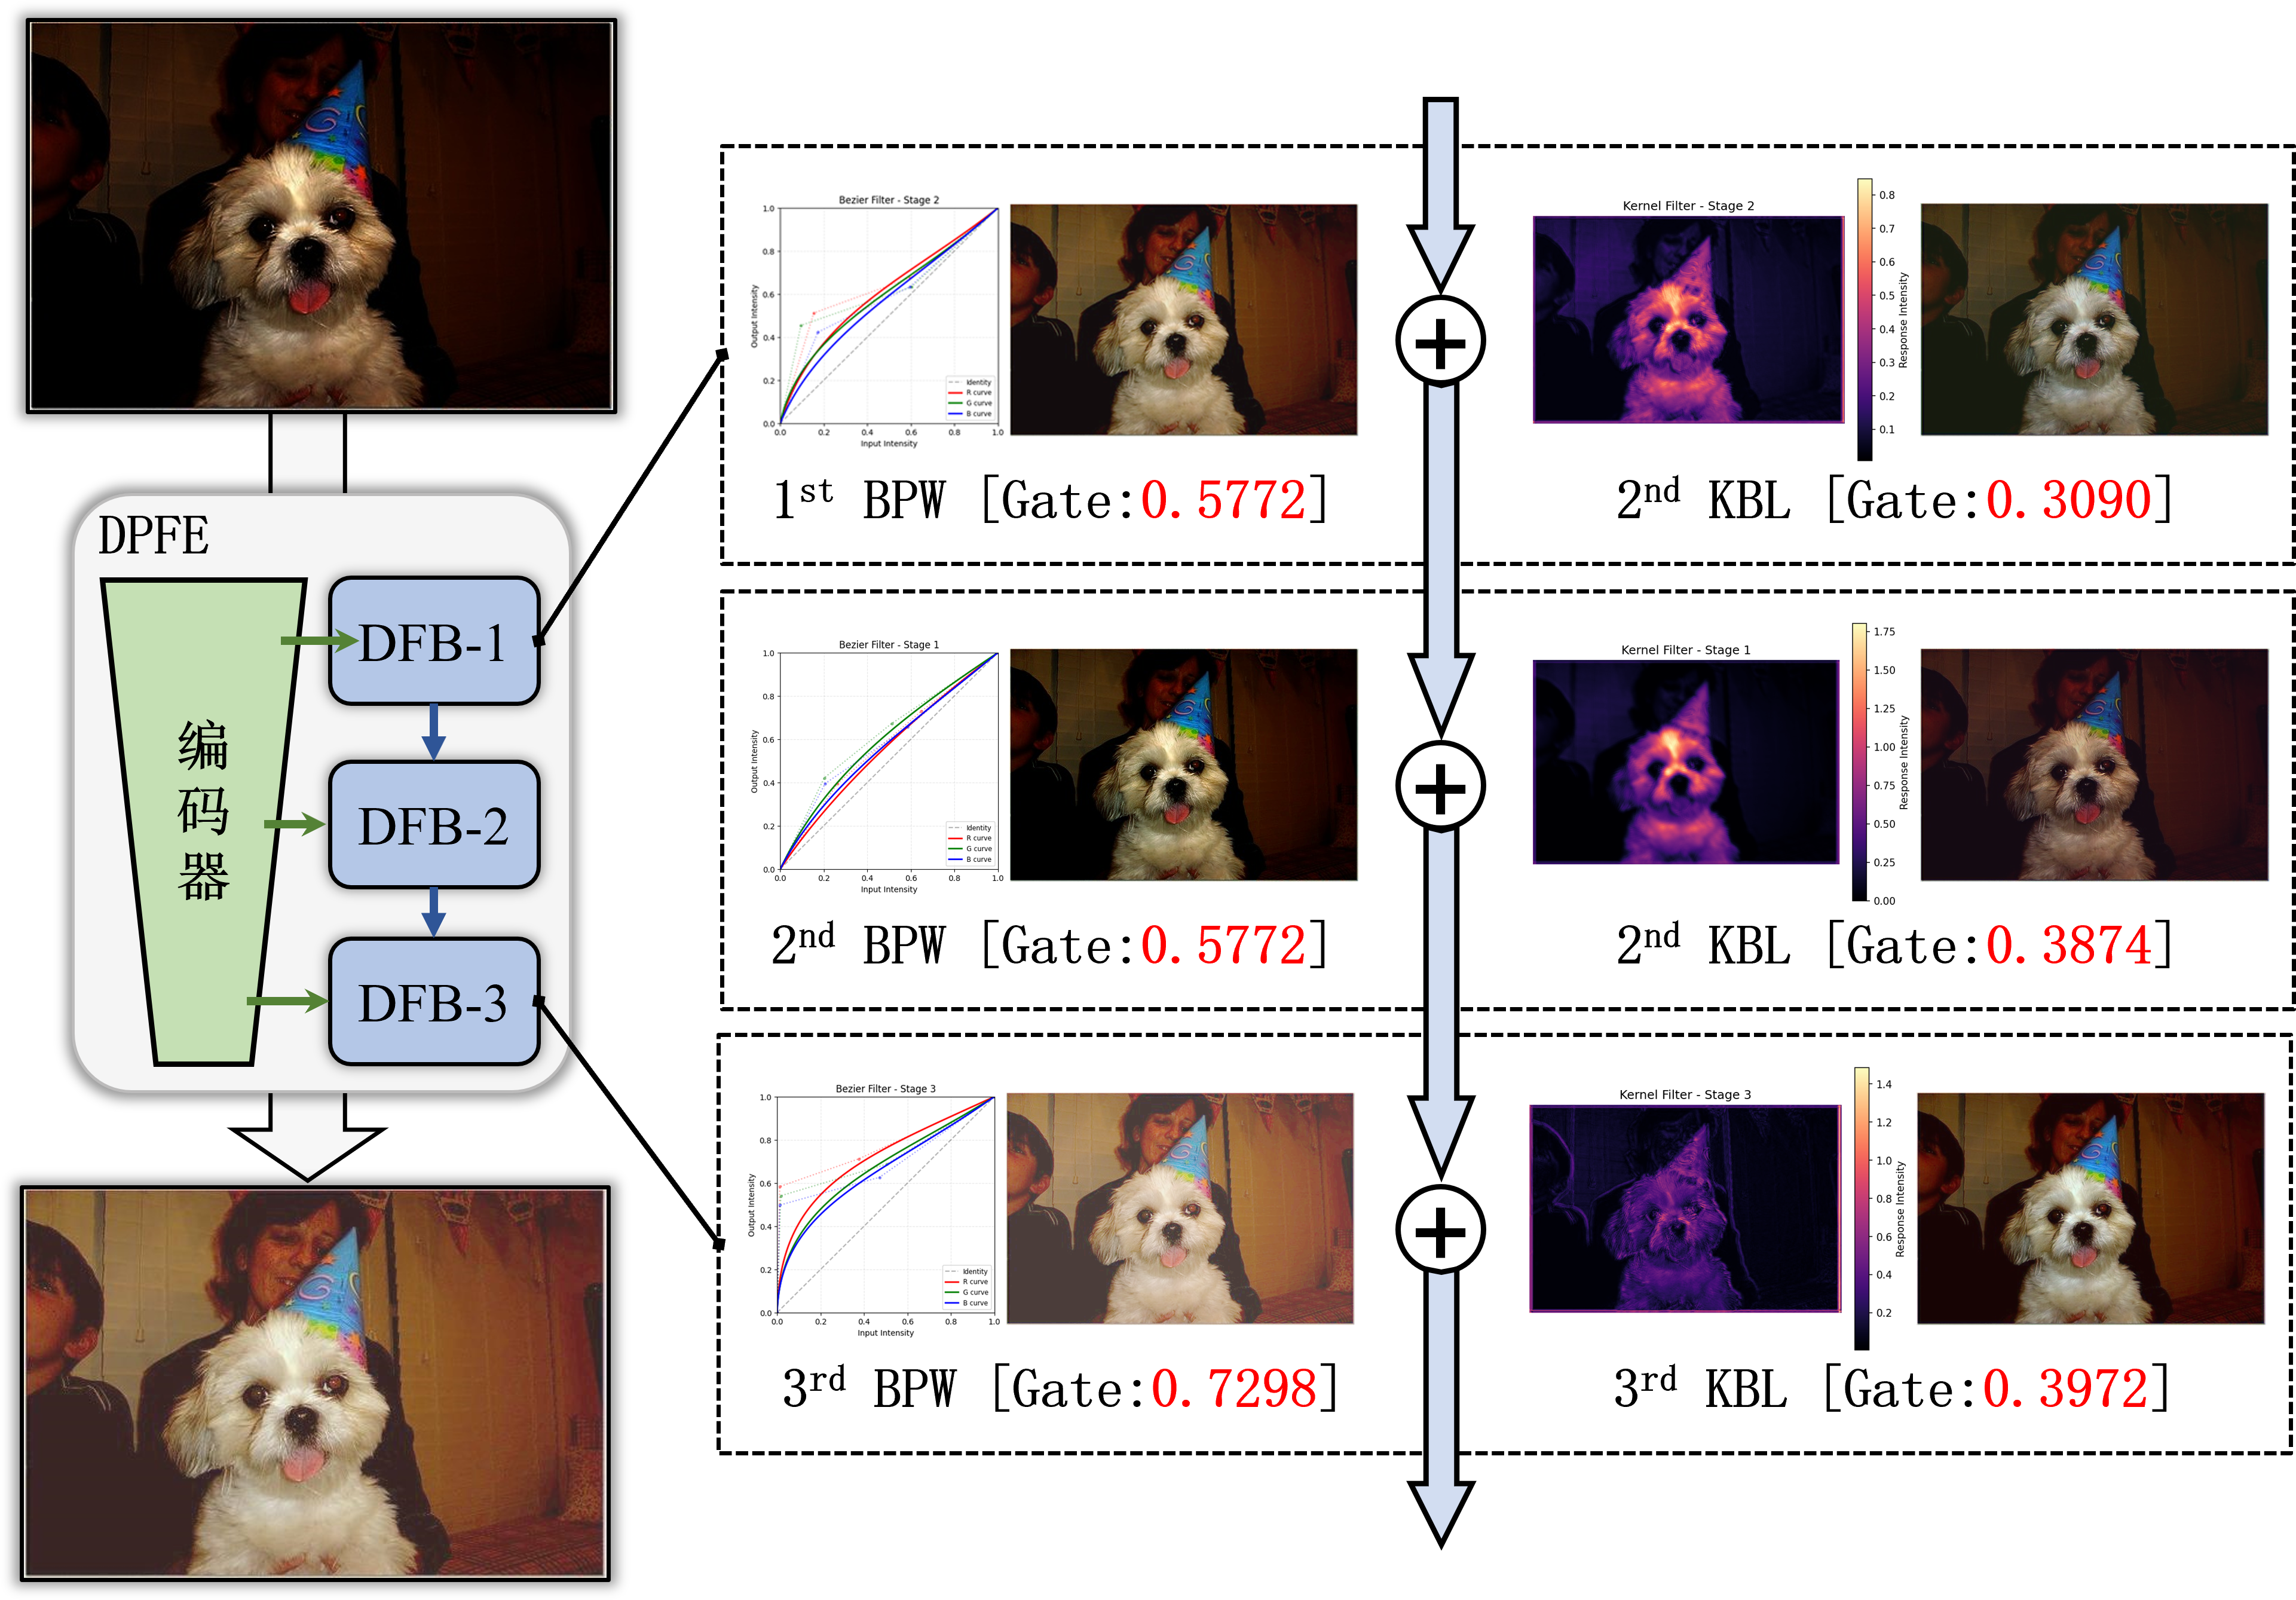
\includegraphics[width=15cm]{chapter3/11.png}
    \caption{\label{fig:ch_3_11}MOT17-05视频序列的跟踪对比}
\end{figure}

如图 \ref{fig:ch_3_11} 所示,在 MOT17-05 序列中,两名行人在移动视角下发生交叉并产生短时遮挡。
在第78帧,穿白衬衫的男性被分配为 ID \#134,此时其前方的短袖女性被部分遮挡;
当遮挡在第80帧解除后,ImprAss-OC 未能正确恢复原有身份假设,
错误地将 ID \#134 分配给短袖女性,并为白衬衫男性重新分配 ID \#141,导致明显的身份切换。

相比之下,DGCTracker 在整个交叉过程中始终保持了白衬衫男性身份的一致性。
其原因在于:即使目标在局部区域内发生遮挡,静态图分支仍能通过邻域内稳定的空间结构关系维持对目标身份的连续建模;
同时,动态图分支在遮挡解除后,能够结合判别性语义特征对候选关联进行重新排序,
从而避免因短时遮挡导致的错误身份继承。该结果表明,DGCTracker 在动态视角与遮挡并存的场景下,具备更强的身份恢复与遮挡鲁棒性。

\textbf{(2) 远距离小目标的稳定跟踪能力 (MOT17-02)}

如图 \ref{fig:ch_3_12} 所示,在 MOT17-02 序列中,目标距离摄像机较远,检测框尺寸较小且外观纹理信息有限。
在第71帧与第73帧,ImprAss-OC 将该黑衣行人稳定跟踪为 ID \#5;
然而在第82帧,尽管检测器仍然成功检测到该目标,ImprAss-OC 却未能完成有效关联,导致轨迹中断,并在第84帧将其误判为新目标(ID \#34)。

DGCTracker 在该场景下始终保持该行人的身份为 ID \#5。
对于远距离小目标而言,单纯依赖外观相似度极易受到特征噪声干扰,
而 DGCTracker 通过图结构建模,将目标嵌入到整体场景的空间与运动上下文中。
当目标在连续帧中发生轻微位置漂移或短时关联不确定时,其在图结构中的相对拓扑关系仍保持连续性,
从而为正确的跨帧关联提供了额外约束。这一结果表明,DGCTracker 在弱外观条件下具备更强的轨迹连续性建模能力。
\begin{figure}[htbp]
    \centering
    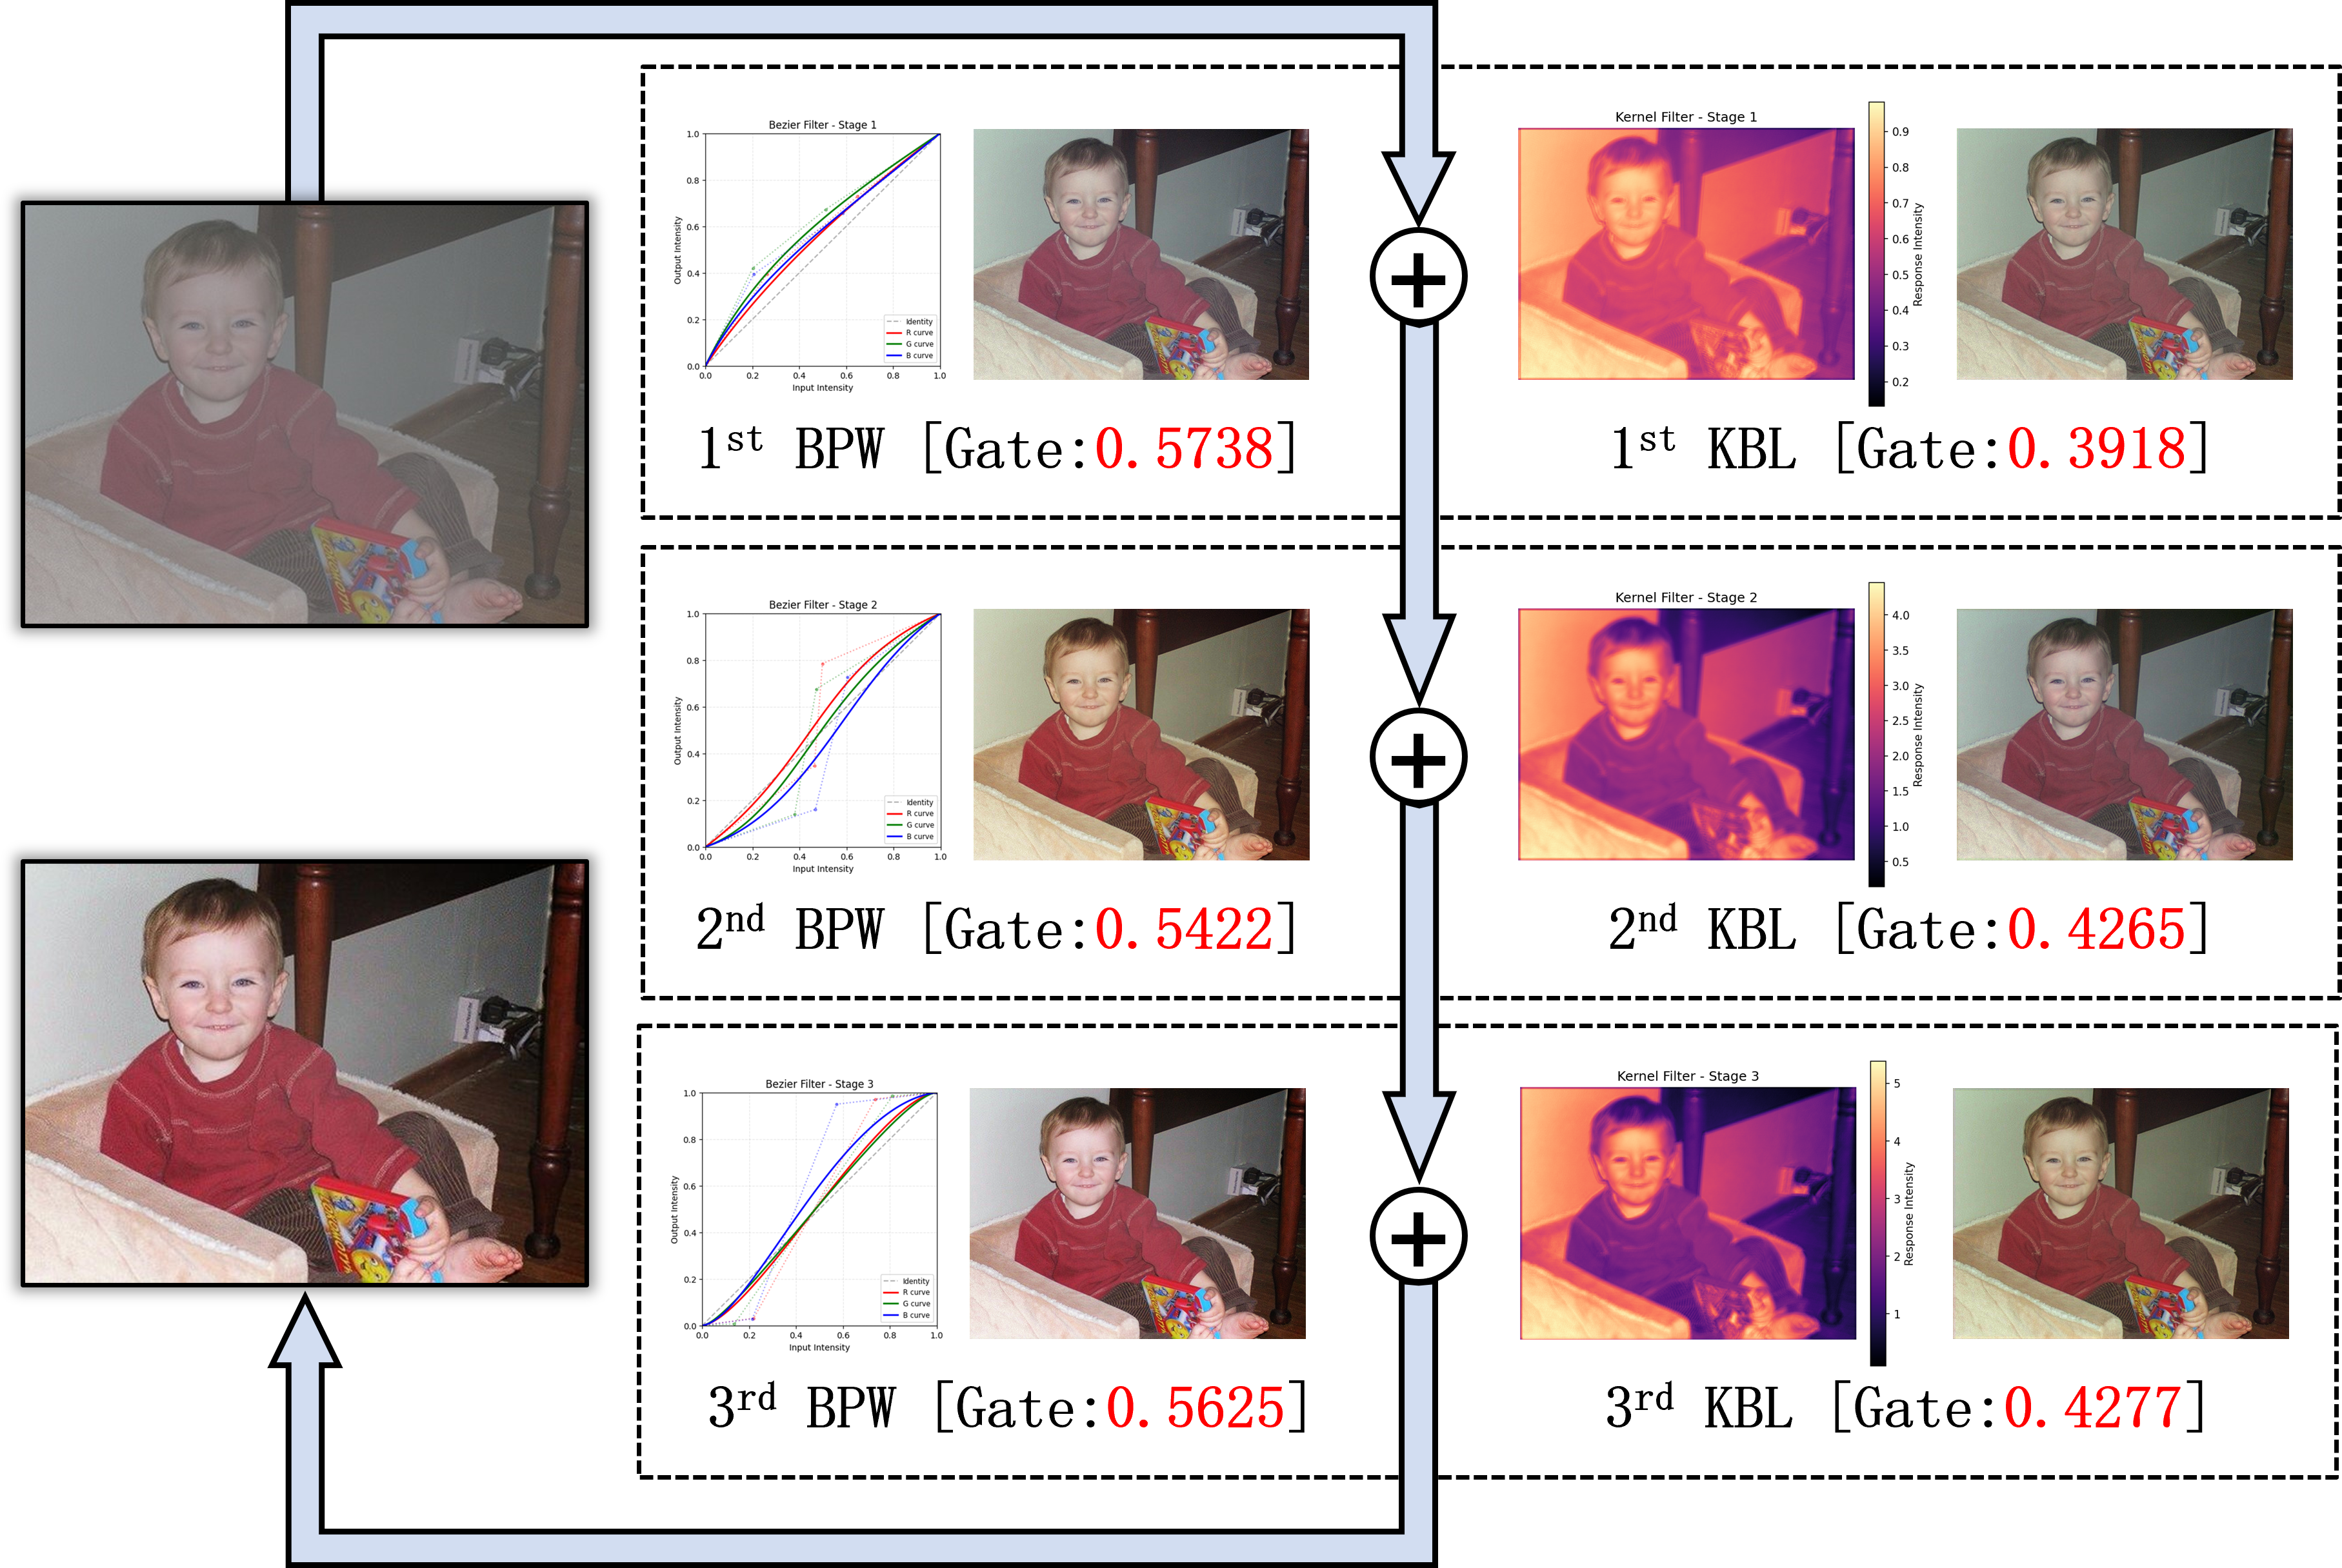
\includegraphics[width=15cm]{chapter3/12.png}
    \caption{\label{fig:ch_3_12}MOT17-02视频序列的跟踪对比}
\end{figure}

\textbf{(3) 密集场景下相似外观的区分能力 (MOT17-04)}

如图 \ref{fig:ch_3_13} 所示,在 MOT17-04 的高密度场景中,两名外观与位置高度相似(均着白色上衣)的行人相继出现。
在第25帧,检测器仅检测到其中一名白衣男性并赋予 ID \#19;
而在第28帧,另一名外观相似的白衣女性进入场景,导致目标间高度混淆。
此时,基于局部关系建模的图方法 GSM 出现身份漂移,将 ID \#19 错误分配给新出现的女性目标。

DGCTracker 在该场景下有效避免了这一问题。
其双图结构通过层次化的特征关系建模,在保持局部空间一致性的同时,
进一步在特征空间中放大相似目标之间的细微差异。
动态图分支通过动态重构邻接关系,迫使网络在嵌入空间中对相似目标进行区分,
从而在新目标出现时为其分配新的身份,并稳定维持原有目标的身份信息。该结果说明,DGCTracker 在密集且外观高度相似的场景中具备更强的判别性建模能力。
\begin{figure}[htbp]
    \centering
    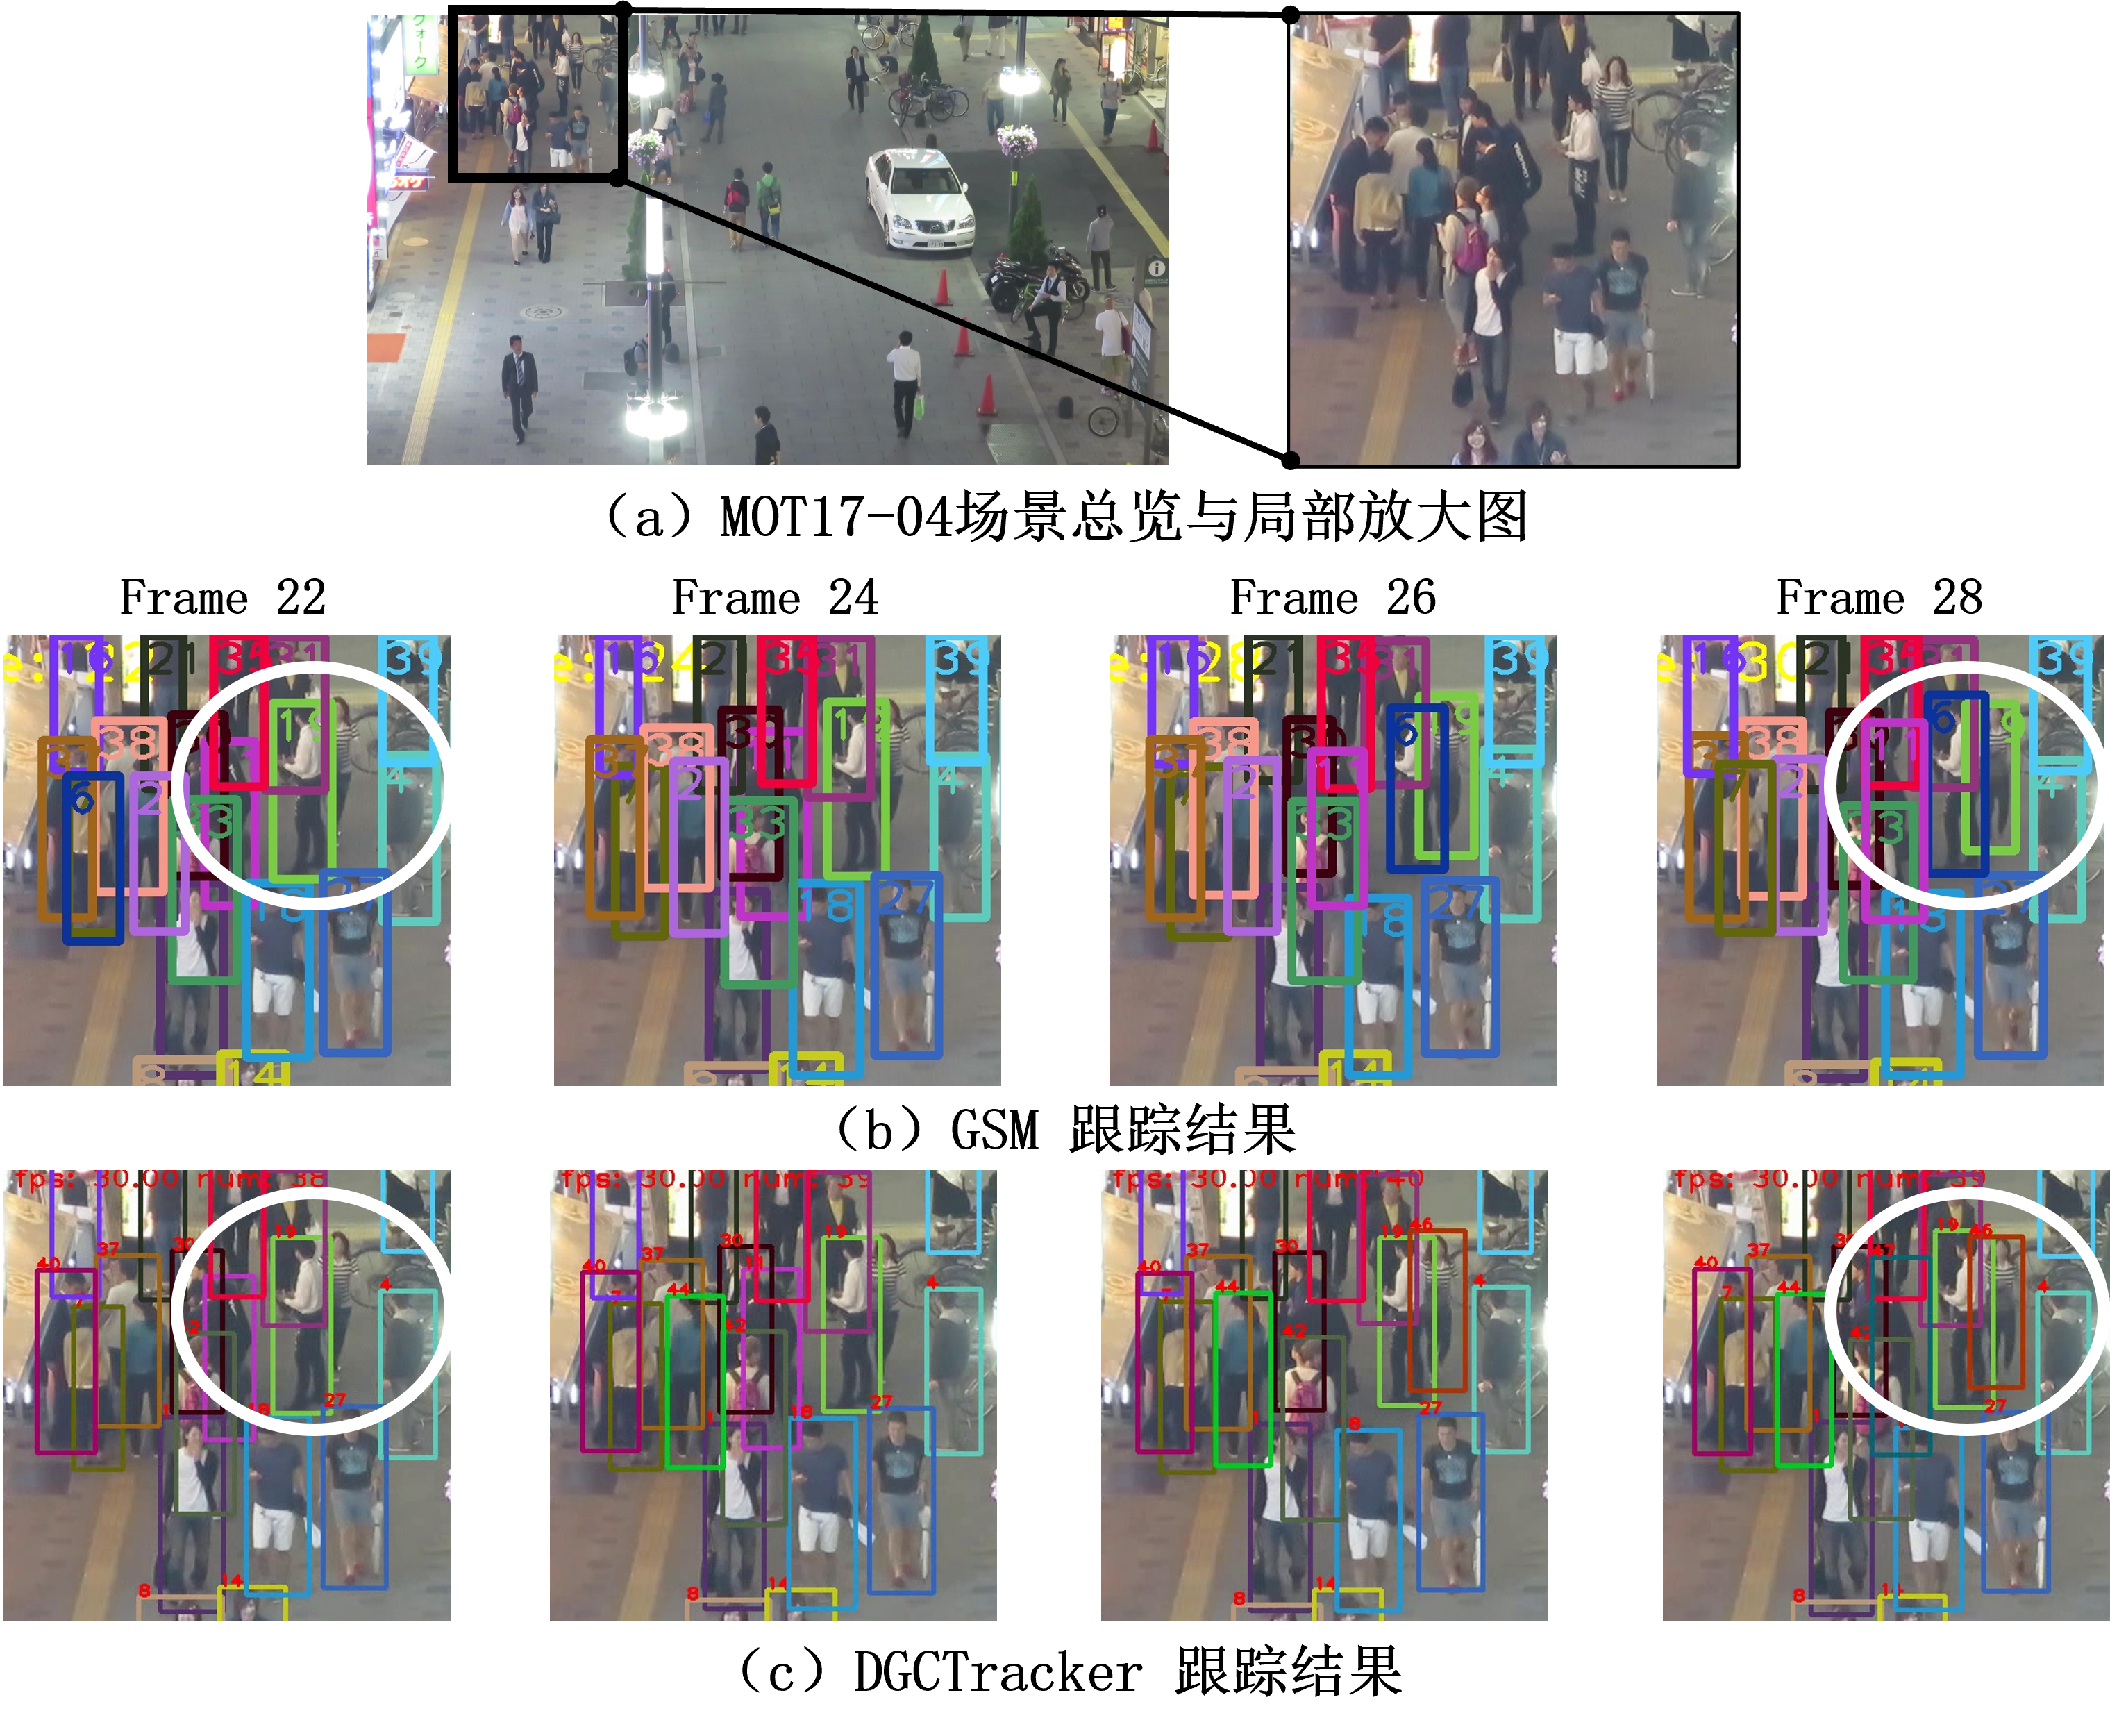
\includegraphics[width=15cm]{chapter3/13.png}
    \caption{\label{fig:ch_3_13}MOT17-04视频序列的跟踪对比}
\end{figure}

通过上述定量与定性对比可以看出,DGCTracker 在目标密集、遮挡频繁以及外观变化显著的复杂场景中,展现出更强的身份保持能力与轨迹稳定性。这一优势主要得益于其基于图神经网络的上下文建模能力,以及在全局约束下进行的跨帧关联优化。

\subsection{消融实验}
\label{subsec:ch3_4_3}
为深入验证 DGCTracker 中各核心组件的有效性及其设计选择的合理性,本节在 MOT17 测试集上进行了系统的消融实验。
实验主要围绕三个方面展开:图拓扑结构的构建方式、图神经网络的结构设计以及数据增强策略。所有实验均保持其他部分与基准模型一致,仅变动待研究的单一变量,以确保结论的可靠性。

\textbf{1. 图拓扑结构的构建方式}

图作为 DGCTracker 中进行关系建模的基础数据结构,其具体构建方式对模型性能具有根本性影响。为了确定最优的构图策略,我们从边的方向性、自环的设置、动态图的度量标准以及邻居数量 $K$ 值四个方面进行了详细的对比实验。

\textbf{(1) 有向图与无向图的对比}

图的边是否具有方向性深刻影响着节点间关系的表达。为此,我们对比了同样基于 $K$ 近邻(KNN)构建的有向图与对应的的无向图的性能差异。图 \ref{fig:ch_3_14} 展示了两种图的拓扑差异。
\begin{figure}[htbp]
    \centering
    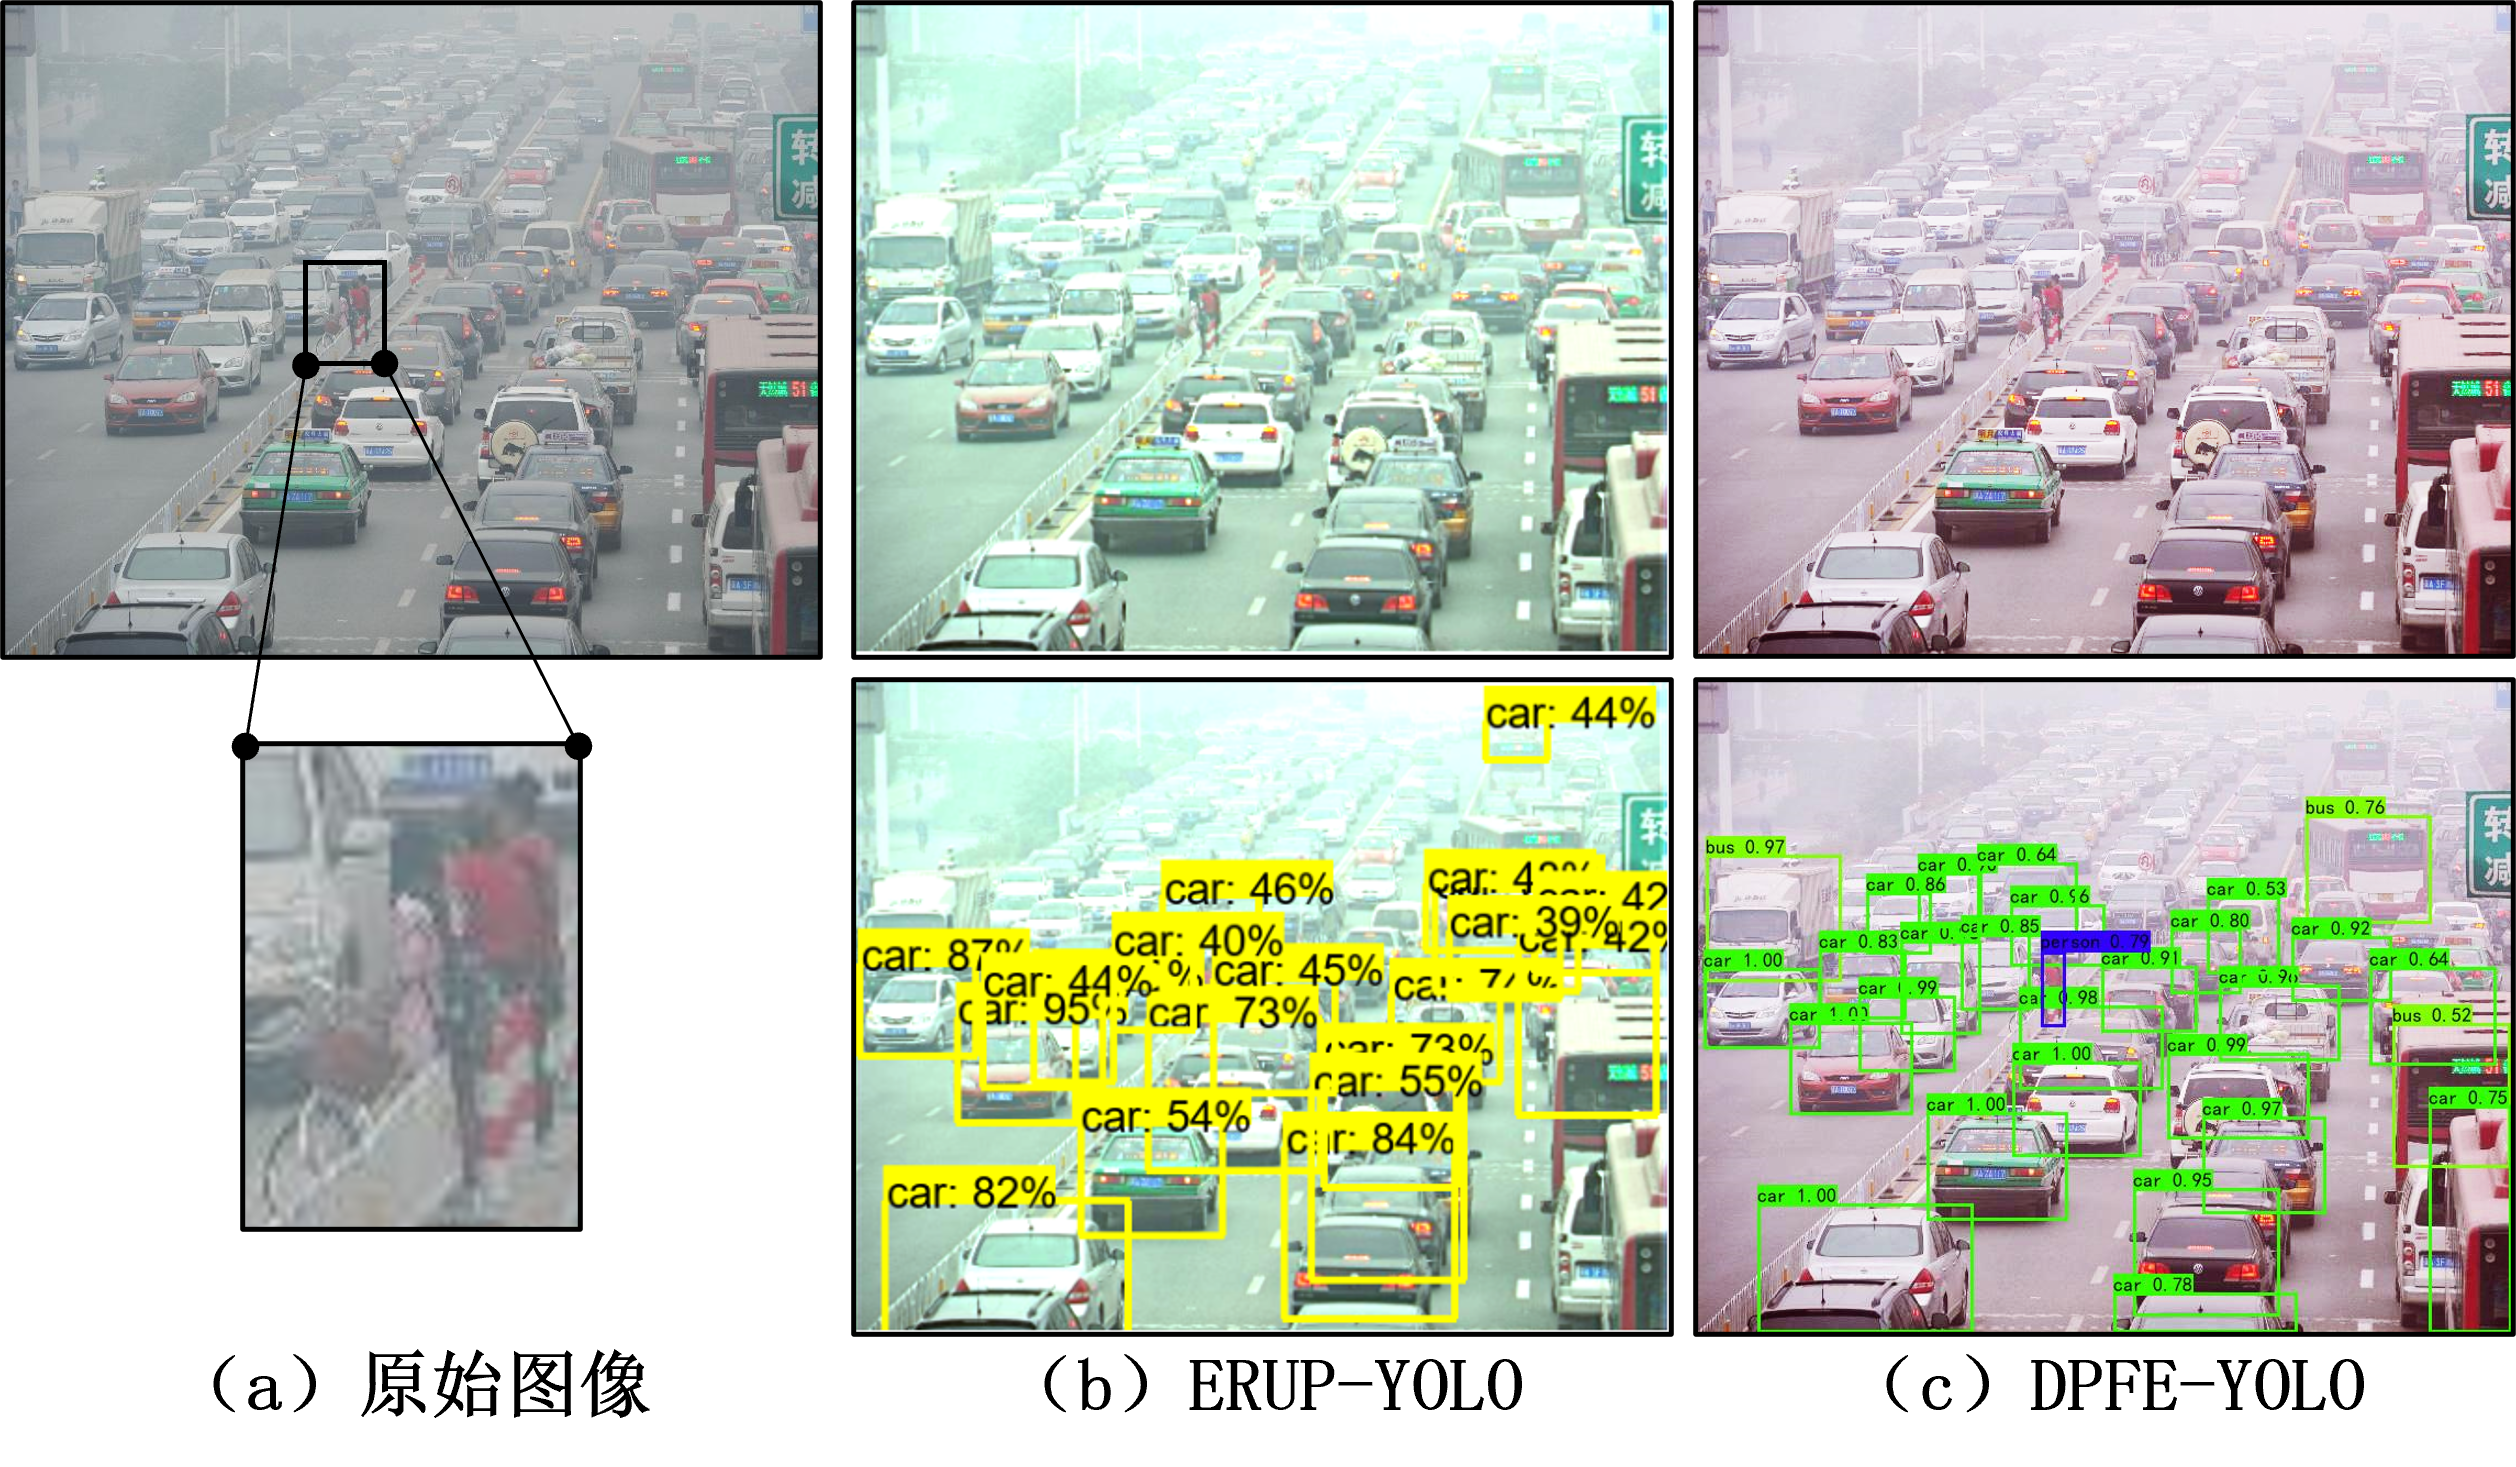
\includegraphics[width=15cm]{chapter3/14.png}
    \caption{\label{fig:ch_3_14}有向图与无向图拓扑结构示意图}
\end{figure}

\begin{table}[htbp]
  \centering
  \caption{有向图与无向图对跟踪性能的影响对比}
  \label{tab:ch_3_4_3_1}
  \resizebox{0.9\linewidth}{!}{
  \begin{tabular}{ccccccccc}
    \toprule
    \textbf{图类型} & \textbf{HOTA} $\uparrow$ & \textbf{DetA} $\uparrow$ & \textbf{AssA} $\uparrow$ & \textbf{IDF1} $\uparrow$ & \textbf{IDR} $\uparrow$ & \textbf{IDP} $\uparrow$ & \textbf{MOTA} $\uparrow$ & \textbf{MOTP} $\uparrow$ \\
    \midrule
    无向图 & 58.18 & \textbf{56.54} & 62.47 & 67.48 & 56.98 & 82.71 & 64.90 & 84.62 \\
    \textbf{有向图 (Ours)} & \textbf{61.65} & 56.42 & \textbf{67.56} & \textbf{72.64} & \textbf{61.25} & \textbf{89.25} & \textbf{65.59} & \textbf{84.67} \\
    \bottomrule
  \end{tabular}
  }
\end{table}

实验结果如表 \ref{tab:ch_3_4_3_1} 所示,采用有向图结构的 HOTA 达到了 61.65,相比无向图(58.18)提升了 3.47\%;而在反映关联质量的 AssA 指标上,提升幅度更是高达 5.09\%。
这是因为多目标跟踪中的特征空间往往是非对称的。例如,基于 KNN 构建邻域时,节点 A 将 B 选为邻居,并不意味着 B 的邻域中一定包含 A(即 $B \in \mathcal{N}(A) \nRightarrow A \in \mathcal{N}(B)$)。
无向图强制对称化这种关系,引入了大量非必要的噪声连接,稀释了关键的拓扑信息。而有向图能够更精确地保留特征空间中的非互惠关系,从而使得消息传递更加纯净有效。

\textbf{(2) 自环结构作用分析}

在确定使用有向图后,我们进一步探究是否为节点添加自环(Self-loop)的影响。自环是指节点指向自身的边,它决定了图卷积在聚合邻域信息时,多大程度上保留节点自身的原始特征。
图 \ref{fig:ch_3_15} 展示了有无自环的结构差异。
\begin{figure}[htbp]
    \centering
    \includegraphics[width=13cm]{chapter3/15.png}
    \caption{\label{fig:ch_3_15}自环结构示意图}
\end{figure}

\begin{table}[htbp]
  \centering
  \caption{自环结构对模型性能的影响}
  \label{tab:ch_3_4_3_2}
  \resizebox{0.9\linewidth}{!}{
  \begin{tabular}{ccccccccc}
    \toprule
    \textbf{配置} & \textbf{HOTA} $\uparrow$ & \textbf{DetA} $\uparrow$ & \textbf{AssA} $\uparrow$ & \textbf{IDF1} $\uparrow$ & \textbf{IDR} $\uparrow$ & \textbf{IDP} $\uparrow$ & \textbf{MOTA} $\uparrow$ & \textbf{MOTP} $\uparrow$ \\
    \midrule
    有向自环图 & 61.36 & 56.40 & 67.17 & 71.08 & 59.94 & 87.29 & \textbf{65.67} & \textbf{84.69} \\
    \textbf{有向无环图(Ours)} & \textbf{61.65} & \textbf{56.42} & \textbf{67.56} & \textbf{72.64} & \textbf{61.25} & \textbf{89.25} & 65.59 & 84.67 \\
    \bottomrule
  \end{tabular}
  }
\end{table}

如表\ref{tab:ch_3_4_3_2}所示,不使用自环的图结构在绝大多数指标上略优于使用自环的版本,尤其在 AssA 和 IDF1 上分别有 0.39 和 1.56 个百分点的提升。
这一结果表明,在本任务的消息传递框架中,强制让节点在每一层都显式地“关注自身”并非必要,甚至可能带来轻微的干扰。
我们的网络结构(如公式\ref{equ:sta_gcn})已通过跳跃连接(即 $^{s}f_1^\beta(\cdot)$ 项)在特征更新时融入了节点自身的历史信息,
这足以保证节点特征的稳定性。省略自环则迫使模型在每一层的消息聚合中,必须更充分地利用来自邻居的有效信息来更新自身,这有助于增强特征对局部上下文的敏感性。

需要指出的是,在极端情况下(如图 \ref{fig:ch_3_15}(c)所示),当当前帧中仅存在单个目标节点时,无环图将退化为不包含任何有效边的孤立节点图,从而导致图卷积操作无法正常执行。
为保证算法在该类场景下的健壮性,本文在工程实现中采用如下策略:当图中节点数为 1 时,默认补充自环边以保证图结构有效;当节点数大于 1 时,则使用有向无环图作为默认配置。

\textbf{(3) 动态图构图方式的选择}

动态图的核心在于基于特征相似度重构邻接关系。我们对比了两种常用的特征度量方式:欧式距离(Euclidean Distance)与余弦相似度(Cosine Similarity)。
\begin{table}[htbp]
  \centering
  \caption{不同特征度量方式下的动态图性能对比}
  \label{tab:ch_3_4_3_3}
  \resizebox{0.9\linewidth}{!}{
  \begin{tabular}{ccccccccc}
    \toprule
    \textbf{度量方式} & \textbf{HOTA} $\uparrow$ & \textbf{DetA} $\uparrow$ & \textbf{AssA} $\uparrow$ & \textbf{IDF1} $\uparrow$ & \textbf{IDR} $\uparrow$ & \textbf{IDP} $\uparrow$ & \textbf{MOTA} $\uparrow$ & \textbf{MOTP} $\uparrow$ \\
    \midrule
    基于欧式距离 & 59.81 & 56.32 & 65.09 & 70.96 & 59.86 & 87.13 & 64.86 & \textbf{84.69} \\
    \textbf{基于余弦距离(Ours)} & \textbf{61.65} & \textbf{56.42} & \textbf{67.56} & \textbf{72.64} & \textbf{61.25} & \textbf{89.25} & \textbf{65.59} & 84.67 \\
    \bottomrule
  \end{tabular}
  }
\end{table}

如表 \ref{tab:ch_3_4_3_3} 所示,基于余弦距离的构图方式显著优于欧式距离(HOTA 提升 1.84\%)。
具体而言,动态图的邻接关系构建依赖于图网络输出的高维节点嵌入特征。
这类特征通过静态图与动态图的级联卷积,已融合了目标的拓扑关系与上下文语义。
在高维空间中,其方向主要编码目标的身份语义与结构关联性,而模长则可能受局部噪声(如遮挡、姿态变化)或特征聚合过程中的冗余信息影响。
欧式距离对方向和模长的敏感性会放大模长噪声的干扰,导致语义相似但模长差异较大的节点被误判为不相关;
而余弦相似度通过归一化操作聚焦于特征向量的方向一致性,能够更精准地捕捉目标间的深层语义关联,因此更适合动态图的邻域搜索任务。

\textbf{(4) 邻居数量 $K$ 值的选择分析}

KNN算法中的邻居数 $K$ 直接决定了图的稀疏程度与计算复杂度。图 \ref{fig:ch_3_16} 则直观展示了在一个包含 14 个节点的轨迹图中,随着 $K$ 值增加,连边拓扑结构的演变过程。
\begin{figure}[htbp]
    \centering
    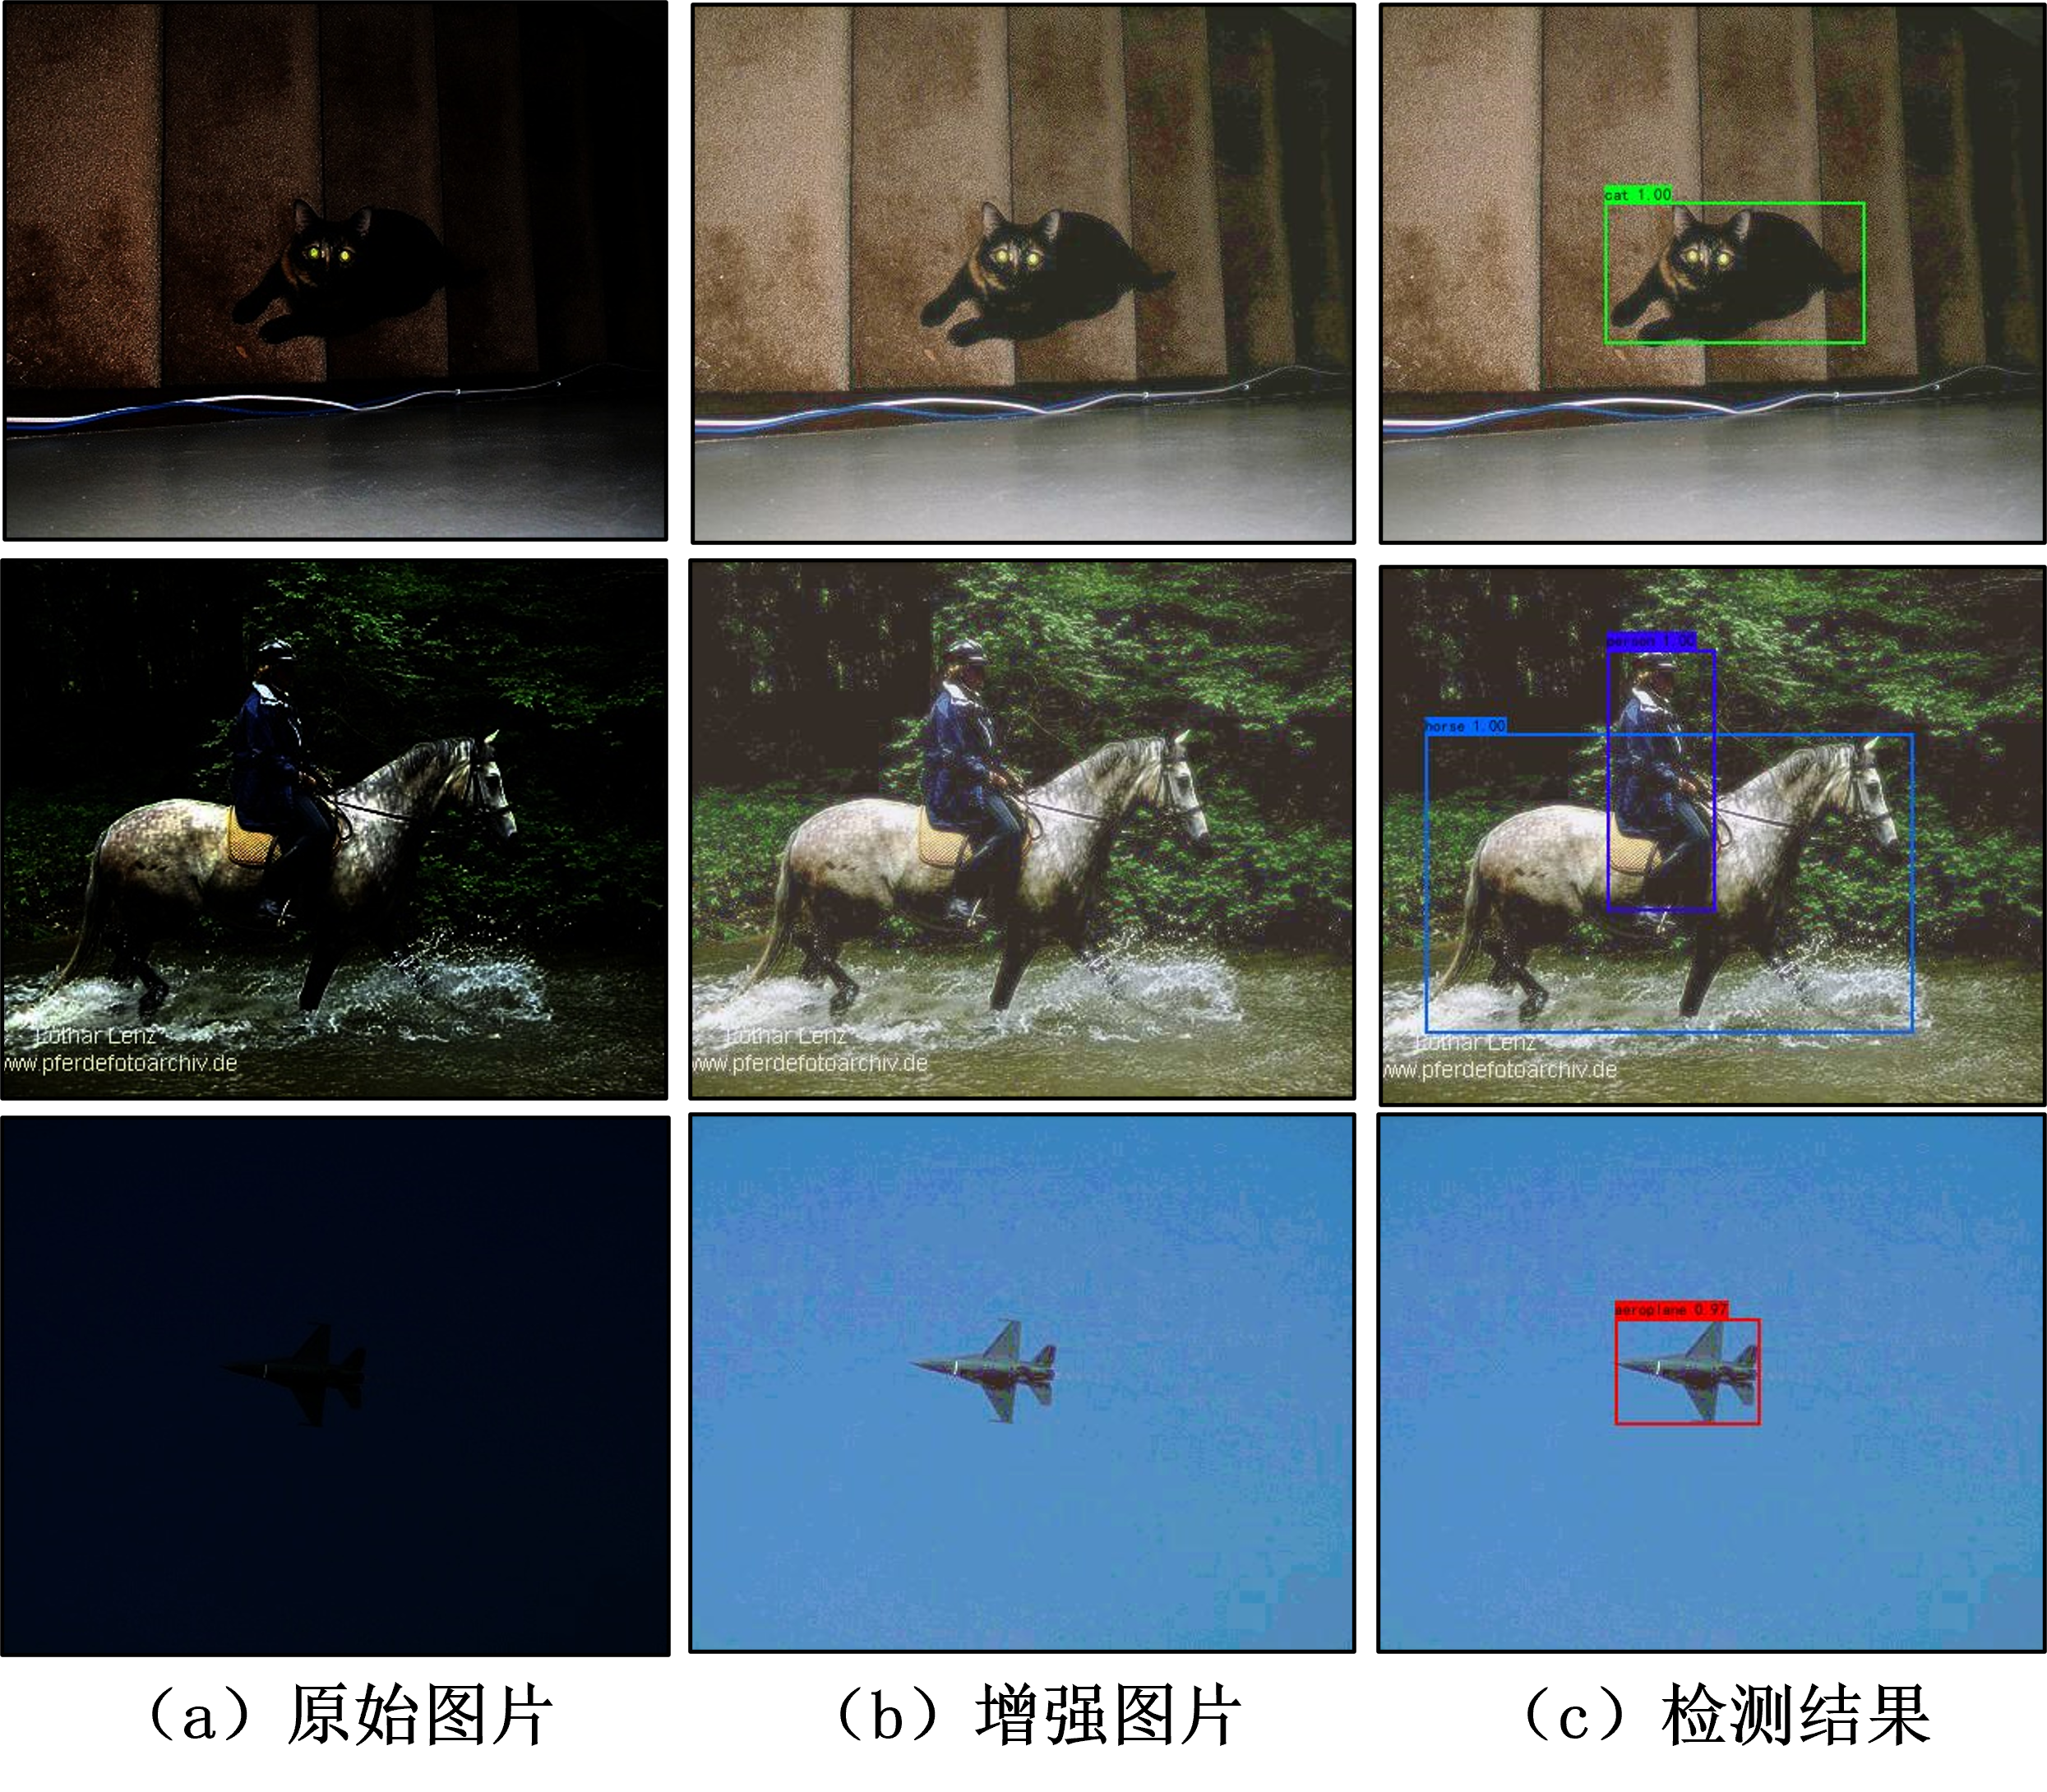
\includegraphics[width=16cm]{chapter3/16.png}
    \caption{\label{fig:ch_3_16}14个节点的图结构随$K$值增加的演变示意图}
\end{figure}

表 \ref{tab:ch_3_4_3_4} 的实验结果表明,当 $K=2$ 时模型取得了最佳的综合性能(HOTA=61.65)。
随着 $K$ 增大,性能先略有波动,在 $K=8$ 之后呈现明显下降趋势,而全连接图的性能最差。这一现象揭示了稀疏图结构的重要性。
过大的 $K$ 值(或全连接)会引入大量非局部的、弱相关的甚至嘈杂的连接,不仅大幅增加计算负担,还会在消息传递过程中引入噪声干扰,导致节点特征表示退化。
$K=2$ 的设置能够在“捕捉必要的局部空间上下文”(如遮挡、群体运动)与“避免冗余连接引入噪声”之间取得了最佳平衡,验证了基于局部性先验进行稀疏构图的合理性。
\begin{table}[htbp]
  \centering
  \caption{邻居数量 $K$ 值对模型性能的消融实验}
  \label{tab:ch_3_4_3_4}
  \resizebox{0.9\linewidth}{!}{
  \begin{tabular}{ccccccccc}
    \toprule
    \textbf{不同K值} & \textbf{HOTA} $\uparrow$ & \textbf{DetA} $\uparrow$ & \textbf{AssA} $\uparrow$ & \textbf{IDF1} $\uparrow$ & \textbf{IDR} $\uparrow$ & \textbf{IDP} $\uparrow$ & \textbf{MOTA} $\uparrow$ & \textbf{MOTP} $\uparrow$ \\
    \midrule
    \textbf{K=2 (Ours)} & \textbf{61.65} & \textbf{56.42} & \textbf{67.56} & 72.64 & 61.25 & 89.25 & 65.59 & 84.67 \\
    4 & 61.50 & 56.40 & 67.37 & \textbf{72.76} & \textbf{61.33} & \textbf{89.44} & \textbf{65.61} & 84.61 \\
    6 & 61.53 & 56.17 & 67.51 & 72.62 & 61.22 & 89.25 & 65.44 & 84.60 \\
    8 & 59.91 & 56.14 & 64.76 & 70.30 & 59.30 & 86.36 & 65.17 & \textbf{84.70} \\
    16 & 60.47 & 56.38 & 65.55 & 70.82 & 59.73 & 86.99 & 64.99 & \textbf{84.70} \\
    64 & 60.76 & 56.03 & 66.29 & 71.05 & 59.92 & 87.28 & 64.94 & 84.69 \\
    全连接图 & 59.94 & 56.23 & 64.76 & 70.24 & 59.24 & 86.28 & 64.96 & 84.66 \\
    \bottomrule
  \end{tabular}
  }
\end{table}

\textbf{2. 图神经网络的结构设计}

在确定了最佳的图拓扑结构后,我们进一步对 DGCTracker 中核心神经网络模块的内部构造进行了消融研究。这部分实验主要探讨了残差连接、聚合函数、归一化策略、网络层数配置以及亲和矩阵融合方式对跟踪性能的影响。

\textbf{(1) 静态图卷积中残差连接的作用}

首先,我们验证静态图卷积中引入残差连接的必要性。
原始模型中,静态图卷积采用如公式\ref{equ:sta_gcn} 所示的结构,
通过将节点自身特征与邻域聚合结果相加,实现对历史信息的显式保留。
对应地,我们构造了一个去除残差项的变体,仅保留邻居消息聚合,同时保持动态图卷积结构不变,其更新形式如下所示:
\begin{equation}
\begin{dcases}
    ^{s}h_i^{\beta} = {^{s}g^\beta}\left(  \max_{j \in \mathcal{N}(i)} {^{s}f_2}^\beta\left( ^{s}z_{ji} ~, \left( ^{s}h_j^{\beta-1} - {^{s}h_i^{\beta-1}} \right) \right) \right) \\
    ^{d}h_i^{\beta} = \max_{j \in \mathcal{N}^{\beta}(i)} {^{d}f^\beta}\left( \left[^{d}h_{i}^{\beta -1} ~\cdot~\left( ^{d}h_j^{\beta-1} - {^{d}h_i^{\beta-1}} \right) \right] \right)
\end{dcases}
\end{equation}

如表 \ref{tab:ch_3_4_3_5} 所示,去除残差连接后,HOTA 指标下降了 2.12\%,AssA 下降显著。
主要原因在于:深层图神经网络普遍面临着过平滑(Over-smoothing)问题,
即随着层数加深,不同节点的特征趋于一致,丧失了区分度。残差连接使得每一层的输出都显式地融合了上一层的输入特征,
保证了节点在聚合邻域信息的同时,不会丢失其该层输入的独特性。这对维持长时跟踪中目标身份的稳定性至关重要。
\begin{table}[htbp]
  \centering
  \caption{静态图卷积中残差连接的消融实验}
  \label{tab:ch_3_4_3_5}
  \resizebox{0.9\linewidth}{!}{
  \begin{tabular}{ccccccccc}
    \toprule
    \textbf{配置} & \textbf{HOTA} $\uparrow$ & \textbf{DetA} $\uparrow$ & \textbf{AssA} $\uparrow$ & \textbf{IDF1} $\uparrow$ & \textbf{IDR} $\uparrow$ & \textbf{IDP} $\uparrow$ & \textbf{MOTA} $\uparrow$ & \textbf{MOTP} $\uparrow$ \\
    \midrule
    无残差连接 & 59.53 & 56.35 & 63.83 & 69.30 & 58.49 & 85.03 & 65.23 & 84.63 \\
    \textbf{有残差连接 (Ours)} & \textbf{61.65} & \textbf{56.42} & \textbf{67.56} & \textbf{72.64} & \textbf{61.25} & \textbf{89.25} & \textbf{65.59} & \textbf{84.67} \\
    \bottomrule
  \end{tabular}
  }
\end{table}

\textbf{(2) 邻域消息聚合方式选择}

接下来,我们对静态图与动态图卷积中的邻居聚合算子进行了消融,将默认的最大池化(max pooling)替换为均值聚合(mean pooling),其对应更新形式如下所示:
\begin{equation}
\begin{dcases}
    ^{s}h_i^{\beta} = {^{s}g^\beta}\left(  \frac{1}{N}\sum_{j \in \mathcal{N}(i)} {^{s}f_2}^\beta\left( ^{s}z_{ji} ~, \left( ^{s}h_j^{\beta-1} - {^{s}h_i^{\beta-1}} \right) \right) \right) \\
    ^{d}h_i^{\beta} = \frac{1}{N}\sum_{j \in \mathcal{N}^{\beta}(i)} {^{d}f^\beta}\left( \left[^{d}h_{i}^{\beta -1} ~\cdot~\left( ^{d}h_j^{\beta-1} - {^{d}h_i^{\beta-1}} \right) \right] \right)
\end{dcases}
\end{equation}

实验结果如表 \ref{tab:ch_3_4_3_6} 所示,Max Pooling 的表现显著优于 Mean Pooling,尤其在 AssA 与 IDF1 指标上分别上升了 4.4 和 3.6 个百分点。
该结果说明,在多目标跟踪任务中,不同邻居对目标关联的贡献并不均衡,最大聚合能够更有效地突出判别性最强的邻居关系,而均值操作则容易引入冗余甚至噪声信息,从而削弱特征的区分性。
\begin{table}[htbp]
  \centering
  \caption{不同聚合函数对模型性能的影响}
  \label{tab:ch_3_4_3_6}
  \resizebox{0.9\linewidth}{!}{
  \begin{tabular}{ccccccccc}
    \toprule
    \textbf{聚合方式} & \textbf{HOTA} $\uparrow$ & \textbf{DetA} $\uparrow$ & \textbf{AssA} $\uparrow$ & \textbf{IDF1} $\uparrow$ & \textbf{IDR} $\uparrow$ & \textbf{IDP} $\uparrow$ & \textbf{MOTA} $\uparrow$ & \textbf{MOTP} $\uparrow$ \\
    \midrule
    Mean Pooling & 58.98 & 55.99 & 63.14 & 69.03 & 58.27 & 84.68 & 65.04 & 84.66 \\
    \textbf{Max Pooling (Ours)} & \textbf{61.65} & \textbf{56.42} & \textbf{67.56} & \textbf{72.64} & \textbf{61.25} & \textbf{89.25} & \textbf{65.59} & \textbf{84.67} \\
    \bottomrule
  \end{tabular}
  }
\end{table}

\textbf{(3) 归一化方式选择}

为了进一步分析特征归一化方式对模型性能的影响,我们对比了 Batch Normalization 与 Graph Normalization 两种策略。
\begin{table}[htbp]
  \centering
  \caption{不同归一化方式的性能对比}
  \label{tab:ch_3_4_3_7}
  \resizebox{0.9\linewidth}{!}{
  \begin{tabular}{ccccccccc}
    \toprule
    \textbf{归一化方式} & \textbf{HOTA} $\uparrow$ & \textbf{DetA} $\uparrow$ & \textbf{AssA} $\uparrow$ & \textbf{IDF1} $\uparrow$ & \textbf{IDR} $\uparrow$ & \textbf{IDP} $\uparrow$ & \textbf{MOTA} $\uparrow$ & \textbf{MOTP} $\uparrow$ \\
    \midrule
    BatchNorm & 61.48 & 56.35 & 67.32 & 71.70 & 60.49 & 88.02 & 64.99 & 84.59 \\
    \textbf{GraphNorm (Ours)} & \textbf{61.65} & \textbf{56.42} & \textbf{67.56} & \textbf{72.64} & \textbf{61.25} & \textbf{89.25} & \textbf{65.59} & \textbf{84.67} \\
    \bottomrule
  \end{tabular}
  }
\end{table}

表 \ref{tab:ch_3_4_3_7} 显示 GraphNorm 取得了略优的结果。这一差异主要源于图结构数据的非独立同分布特性。
相比 BatchNorm 依赖 batch 维度统计信息,GraphNorm 能够针对每个图实例自适应地调整特征分布,
更适合处理节点数量动态变化的图结构数据。因此,在最终模型中,我们采用 GraphNorm 作为默认归一化方式。

\textbf{(4) 静态与动态图卷积的层数配置}

静态图卷积(s)与动态图卷积(d)的层数配置直接影响模型的感受野和表征能力。如表\ref{tab:ch_3_4_3_8}所示,随着层数的增加(从1s+1d到3s+2d),模型性能呈现单调提升的趋势。
“3s+2d” 的配置取得了最优结果。
\begin{table}[htbp]
  \centering
  \caption{不同图卷积层数配置下的模型性能}
  \label{tab:ch_3_4_3_8}
  \resizebox{0.9\linewidth}{!}{
  \begin{tabular}{ccccccccc}
    \toprule
    \textbf{配置} & \textbf{HOTA} $\uparrow$ & \textbf{DetA} $\uparrow$ & \textbf{AssA} $\uparrow$ & \textbf{IDF1} $\uparrow$ & \textbf{IDR} $\uparrow$ & \textbf{IDP} $\uparrow$ & \textbf{MOTA} $\uparrow$ & \textbf{MOTP} $\uparrow$ \\
    \midrule
    1s + 1d & 57.55 & 55.54 & 59.88 & 66.73 & 56.23 & 82.04 & 64.14 & 84.24 \\
    2s & 59.01 & 54.97 & 63.58 & 69.23 & 58.69 & 84.39 & 62.88 & 84.47 \\
    2s + 1d & 60.43 & 56.08 & 65.33 & 71.45 & 60.21 & 87.85 & 65.35 & 84.60 \\
    3s & 59.67 & 55.79 & 64.01 & 70.17 & 59.13 & 86.29 & 65.04 & 84.52 \\
    3s + 1d & 60.80 & 56.27 & 65.88 & 71.48 & 60.29 & 87.76 & 65.30 & 84.61 \\
    \textbf{3s + 2d (Ours)} & \textbf{61.65} & \textbf{56.42} & \textbf{67.56} & \textbf{72.64} & \textbf{61.25} & \textbf{89.25} & \textbf{65.59} & \textbf{84.67} \\
    \bottomrule
  \end{tabular}
  }
\end{table}

这一现象说明:
1)静态图与动态图具有互补性,二者结合优于单一结构;
2)足够的网络深度是必要的。更深的静态图卷积能整合多跳空间邻居的信息,
捕获更广泛的几何上下文;而更深的动态图卷积则允许节点在特征空间中进行多轮迭代的相似性匹配与特征“推离”,
从而学习到更具判别力的表示。这验证了本文设计的层次化特征提取架构的有效性。

\textbf{(5) 亲和矩阵的多模态特征融合}

最后,我们探究了在计算最终亲和矩阵时,不同信息源的贡献度。我们对比了仅使用图节点嵌入(Node)、融合表观特征(Node+App)、融合几何IOU(Node+HIoU)以及三者融合(Triple)的效果。
\begin{table}[htbp]
  \centering
  \caption{不同特征融合策略对亲和矩阵质量的影响}
  \label{tab:ch_3_4_3_9}
  \resizebox{0.9\linewidth}{!}{
  \begin{tabular}{ccccccccc}
    \toprule
    \textbf{模态选择} & \textbf{HOTA} $\uparrow$ & \textbf{DetA} $\uparrow$ & \textbf{AssA} $\uparrow$ & \textbf{IDF1} $\uparrow$ & \textbf{IDR} $\uparrow$ & \textbf{IDP} $\uparrow$ & \textbf{MOTA} $\uparrow$ & \textbf{MOTP} $\uparrow$ \\
    \midrule
    Node Only & 48.65 & 51.56 & 46.26 & 54.01 & 45.27 & 66.95 & 56.50 & 82.98 \\
    Node + App & 53.78 & 54.01 & 53.88 & 61.41 & 51.69 & 75.64 & 61.76 & 84.02 \\
    Node + HIoU & 60.34 & 56.15 & 65.05 & 70.99 & 59.87 & 87.18 & 65.28 & 84.54 \\
    \textbf{Triple (Ours)} & \textbf{61.65} & \textbf{56.42} & \textbf{67.56} & \textbf{72.64} & \textbf{61.25} & \textbf{89.25} & \textbf{65.59} & \textbf{84.67} \\
    \bottomrule
  \end{tabular}
  }
\end{table}

表 \ref{tab:ch_3_4_3_9} 表明单一信息源难以支撑鲁棒的跨帧关联。
仅使用节点嵌入时,模型在 AssA 和 IDF1 上表现较差;
引入外观或几何信息后性能显著提升,其中 Node+HIoU 相比 Node+App 取得更大增益,
说明几何一致性在多目标跟踪中具有更强的约束能力。
最终,三种信息联合使用时达到最优结果,验证了本文在亲和建模阶段引入多模态融合策略的合理性与必要性。

\textbf{3. 数据增强策略}

在训练深度图神经网络时,通过数据增强模拟复杂场景是防止模型过拟合、提升泛化能力的关键手段。
正如\ref{subsec:ch3_2_4}节所述,我们引入了三种针对性的数据增强策略,旨在模拟检测器噪声、非典型运动以及不完整的轨迹片段。为了验证这套组合策略的必要性,我们将模型在“未启用”与“启用”数据增强条件下的性能进行了对比。
\begin{table}[htbp]
  \centering
  \caption{数据增强策略对模型追踪性能的影响}
  \label{tab:ch_3_4_3_10}
  \resizebox{0.9\linewidth}{!}{
  \begin{tabular}{ccccccccc}
    \toprule
    \textbf{配置} & \textbf{HOTA} $\uparrow$ & \textbf{DetA} $\uparrow$ & \textbf{AssA} $\uparrow$ & \textbf{IDF1} $\uparrow$ & \textbf{IDR} $\uparrow$ & \textbf{IDP} $\uparrow$ & \textbf{MOTA} $\uparrow$ & \textbf{MOTP} $\uparrow$ \\
    \midrule
    w/o Augmentation & 59.67 & 55.72 & 64.11 & 69.60 & 58.85 & 85.16 & 64.58 & 84.54 \\
    \textbf{w/ Augmentation (Ours)} & \textbf{61.65} & \textbf{56.42} & \textbf{67.56} & \textbf{72.64} & \textbf{61.25} & \textbf{89.25} & \textbf{65.59} & \textbf{84.67} \\
    \bottomrule
  \end{tabular}
  }
\end{table}

如表\ref{tab:ch_3_4_3_10}所示,引入数据增强策略后,模型在所有关键指标上均获得了显著提升。其中,综合性能指标 HOTA 提升了1.98个百分点,关联精度指标 AssA 提升最为明显,达3.45个百分点,身份保持指标 IDF1 也提升了3.04个百分点。这一结果充分证明了数据增强策略的有效性。

\section{本章小结}
\label{sec:ch3_5}

本章围绕在线多目标跟踪中的核心难点——在目标密集、遮挡频繁与外观相似的复杂场景下保持稳定的跨帧身份一致性——提出了一种双图协同关联的在线跟踪器 DGCTracker。
不同于传统跨帧稠密构图并进行边分类的范式,本文将数据关联重新建模为帧内图表征学习与跨图匹配问题:分别对历史轨迹集合与当前检测集合进行稀疏构图,通过图神经网络学习包含上下文信息的节点嵌入,再基于节点嵌入相似性完成跨帧匹配,从而在降低计算冗余的同时增强关联判别能力。

具体而言,DGCTracker 采用 KNN 策略构建稀疏拓扑,并设计静态图卷积与动态图卷积的级联结构:静态分支在固定空间邻域内聚合几何先验以刻画稳定的局部结构关系,动态分支基于特征空间相似性动态重构邻接关系以挖掘语义层面的判别差异与潜在长程依赖。
在匹配阶段,本文进一步融合图上下文相似度、外观相似度与几何一致性(HIoU)构建多模态亲和,并引入 Sinkhorn 可微归一化实现端到端的软指派优化,推理阶段结合匈牙利算法得到满足互斥约束的离散匹配结果。
在此基础上,本章还设计了与关联模块深度耦合的三阶段轨迹管理机制,实现轨迹的生成、维持与终止,从而提升系统面对漏检、遮挡与噪声检测时的稳定性。

实验部分在 MOT16/17 的本地划分上对方法进行了系统验证。
与多种先进方法的对比结果表明,DGCTracker 在 HOTA、AssA 与 IDF1 等关键指标上取得了具有竞争力的性能,尤其在关联一致性相关指标上表现突出;可视化对比进一步说明其在交叉遮挡、远距离小目标以及密集相似人群等挑战场景下能够有效抑制身份漂移并维持轨迹连续性。
此外,消融实验从图拓扑设计、图网络结构配置与数据增强策略等方面验证了各组件的必要性与合理性,证明静态/动态图协同建模与多模态亲和融合对提升关联质量具有显著贡献。

综上,本章提出的 DGCTracker 为在线多目标跟踪提供了一种高效且鲁棒的图关联范式,为后续进一步探索更强的时序建模、更大规模场景的实时部署与跨数据集泛化能力奠定了方法基础。